%   % !TEX root = ../../VIII,3_Rahmen-TeX_8-1.tex
%
%
%   Band VIII, 3 N.~??A22/??Y\textsubscript{1}
%   Signatur/Tex-Datei: LH_37_03_073-074
%   RK-Nr. 60203
%   Überschrift: De la resistence des solides
%   Datierung: [Ende Januar bis März/April 1683]
%   WZ: 803001 = RK-WZ 134 = Krone auf Ring mit Ross, Gegenmarke AB (eins)
%.  SZ: PlusMinus und MinusPlus (insgesamt: drei Vorkommnisse)
%.  Bilddateien (PDF): LH_37_03_073-074_d01; LH_37_03_073-074_d02; LH_37_03_073-074_d03; LH_37_03_073-074_d04; LH_37_03_073-074_d05; LH_37_03_073-074_d06; LH_37_03_073-074_d07; LH_37_03_073-074_d08; LH_37_03_073-074_d09; LH_37_03_073-074_d10; LH_37_03_073-074_d11; LH_37_03_073-074_d012 (insgesamt: zwölf)
%
%
\selectlanguage{ngerman}%
\frenchspacing%
%
\begin{ledgroupsized}[r]{120mm}
\footnotesize
\pstart
\noindent\textbf{Überlieferung:}
\pend
\end{ledgroupsized}
\begin{ledgroupsized}[r]{114mm}
\footnotesize
\pstart \parindent -6mm
\makebox[6mm][l]{\textit{L}}%
Konzept: LH XXXVII 3 Bl.~73\textendash74.
Ein Bogen 2\textsuperscript{o}.
Ein Wasserzeichen auf Bl.~73 mit Gegen\-marke auf Bl. 74:
Papier aus dem Harz.
Vier stark bearbeitete Seiten.
Abriss am unteren Rand von Bl.~73 mit geringfügigem Textverlust.
\pend
\end{ledgroupsized}
%
% \vspace*{5mm}
% \begin{ledgroup}
% \footnotesize
% \pstart
% \noindent\textbf{Datierungsgründe}:
% Terminus post quem (vermutlich): Empfang von Mariottes Brief an Leibniz vom 25 Januar 1683, dem Mariotte seine \textit{Dissertation sur la resistance des solides pour faire voir que Galilée n’a pas bien expliqué la resistance des solides fichés perpendiculairement dans un mur quand on les tire de travers} beigelegt hatte (\textit{LSB} III,~3 N.~437\cite{01231}).\\
%Terminus ante quem (vermutlich): Leibnizens Brief an Mariotte von März/April 1683 (\textit{LSB} III,~3 N.~456\cite{01262}), in dem Ergebnisse dargestellt werden, wie sie in N.~??A22/Y.1 errungen werden: an erster Stelle die Korrektur von Mariottes Bestimmung des Verhältnisses zwischen Bruch- und Zugfestigkeit.\\
% WZ auf Bl. 73: 803001 = RK-WZ 134 = Krone auf Ring mit Ross, Gegenmarke AB (wohl aus dem Harz).\\
% \pend
% \end{ledgroup}
%
\selectlanguage{latin}%
\frenchspacing%
%
%
\vspace{8mm}
%
%
\count\Bfootins=1200
\count\Afootins=1200
\count\Cfootins=1200
%
%
\pstart%
\normalsize%
\noindent%
%
\lbrack73~r\textsuperscript{o}\rbrack% Blatt 73r
%%    %%    %%    %%    A C H T U N G   G E T R I X T    !!    !!    !!    !!
\edtext{}{%
{\xxref{LH_37_03_073r_Ueberschrift-1}{LH_37_03_073r_Ueberschrift-2}}
{%
\lemma{\textit{Neben der Überschrift:}}\Afootnote{%
Excerpta jam sunt ex his meliora et distinctius scripta.\textsuperscript{\lbrack a\rbrack}\\%
\protect\index{Sachverzeichnis}{excerptum}%
\newline%
\footnotesize{\textsuperscript{\lbrack a\rbrack} Excerpta \lbrack...\rbrack\ scripta:
Gemeint ist vermutlich der Entwurf N.~14\textsubscript{2} \textit{De firmitate corporum}, welcher von N.~14\textsubscript{1} herrührt.
Siehe hierzu oben, S.~\refpassage{LH_37_03_073r_ExcerptaMeliora_luzgw-1}{LH_37_03_073r_ExcerptaMeliora_luzgw-2}.\vspace{-2.0em}}}}}
%
\pend%
%
%
% Überschrift
\pstart%
\centering%
De\edlabel{LH_37_03_073r_Ueberschrift-1} la Resistence des solides\edlabel{LH_37_03_073r_Ueberschrift-2}%
\protect\index{Sachverzeichnis}{resistance des solides}
\pend%
\vspace{0.5em}%
%
% \newpage%
\pstart%
\noindent%
Sit
\edtext{in
\edtext{fig.~1}{\lemma{fig.~1}\Cfootnote{%
Das Diagramm \lbrack\textit{Fig.~1}\rbrack\ auf S.~\pageref{LH_37_03_073r_Fig.1}.}}%
}{%
\lemma{in}\Bfootnote{%
\hspace{-0,5mm}fig.~1 \textit{erg.~L}}}%
\protect\index{Sachverzeichnis}{figura}
%
\edtext{trabs\protect\index{Sachverzeichnis}{trabs infixa}
muro\protect\index{Sachverzeichnis}{murus} verticali horizontaliter infixa,
cujus sectio \textit{ABC}.\protect\index{Sachverzeichnis}{sectio trabis}}{%
\lemma{trabs}\Bfootnote{%
\textit{(1)}~\textit{ABC} \textit{(2)}~muro verticali
\textit{(a)}~\textit{AB}
\textit{(b)}~horizontaliter infixa, cujus sectio \textit{ABC}.%
~\textit{L}}}
%
Abstrahamus animum\protect\index{Sachverzeichnis}{animus}
a pondere ipsius trabis,\protect\index{Sachverzeichnis}{pondus trabis}
et sub extremitatem \textit{C} appendamus
\edtext{pondus \textit{D}.\protect\index{Sachverzeichnis}{pondus appensum}
Quaeritur,}{%
\lemma{pondus}\Bfootnote{%
\textbar~novum \textit{gestr.}~%
\textbar\ \textit{D}. Quaeritur,%
~\textit{L}}}
%
quae sit\textso{ ratio ponderis \textit{D} }%
quod trabem in communi sectione cum muro \textit{AB} rumpere
\edtext{potest, nisu\protect\index{Sachverzeichnis}{nisus ponderis}
qui sit ipsi muro}{%
\lemma{potest,}\Bfootnote{%
\textit{(1)}~ad
\textit{(2)}~nisu
\textit{(a)}~ad mu
\textit{(b)}~qui sit ipsi muro%
~\textit{L}}}
%
parallelus;\protect\index{Sachverzeichnis}{nisus rumpendi parallelus}
\edtext{ad\textso{ pondus}}{%
\lemma{ad}\Bfootnote{%
\hspace{-0,5mm}\textbar~ad \textit{streicht Hrsg.}~\textbar\ \textso{pondus}~\textit{L}}}%
%
\textso{ \textit{E} }%
\protect\index{Sachverzeichnis}{pondus evellens}%
quod trabem directe ex muro evelleret\lbrack,\rbrack\
nisu
\edtext{scilicet}{%
\lemma{scilicet}\Bfootnote{%
\textit{erg.~L}}}
%
qui sit ad murum \edlabel{LH_37_03_073r1}perpendicularis.%
\protect\index{Sachverzeichnis}{nisus evellendi perpendicularis}%
\protect\index{Sachverzeichnis}{murus}%
\protect\index{Sachverzeichnis}{trabs infixa}%
%
\edtext{}{{\xxref{LH_37_03_073r1}{LH_37_03_073r2}}\lemma{perpendicularis.}\Bfootnote{%
\textit{(1)}~Manifestum est resistentiam
\textit{(2)}~Ad hanc rem%
~\textit{L}}}
\pend%
%
\pstart%
Ad hanc rem\edlabel{LH_37_03_073r2}
explicandam cum sit partim physica\protect\index{Sachverzeichnis}{res physica}
partim Mathematica\protect\index{Sachverzeichnis}{res mathematica}
opus est hypothesibus quibusdam,\protect\index{Sachverzeichnis}{hypothesis duplex}
% \edtext{}{%
% \lemma{explicandam}\Bfootnote{%
% \textit{(1)}~Hypothe
% \textit{(2)}~cum sit \lbrack...\rbrack\ est hypothesibus% partim physica partim Mathematica opus
% ~\textit{L}}}
%
ut reducatur quaestio ad terminos Matheseos purae.\protect\index{Sachverzeichnis}{mathesis pura}
\edlabel{LH_37_03_073r_zweiHypothesen_ldifug-1}%
Et quidem duplex fieri potest hypothesis,\protect\index{Sachverzeichnis}{hypothesis duplex}
vel enim corpus trabis solidae consideramus tanquam
\edtext{rigidum,\protect\index{Sachverzeichnis}{corpus trabis rigidum}\protect\index{Sachverzeichnis}{corpus trabis tensile}
vel tanquam tensile.\edlabel{LH_37_03_073r_zweiHypothesen_ldifug-2}}{%
\lemma{rigidum,}\Bfootnote{%
\textit{(1)}~ita ut uno eodemque momento
\textit{(2)}~vel tanquam tensile.%
~\textit{L}}}
\pend%
%
%
% \vspace*{1.0em}%
% \centerline{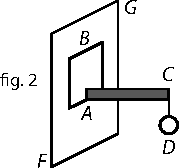
\includegraphics[width=0.28\textwidth]{gesamttex/edit_VIII,3/images/LH_37_03_073-074_d02.pdf}}%\\
% \vspace*{0.0em}
% \centerline{\lbrack\textit{Fig.~2}\rbrack}\label{LH_37_03_073r_Fig.2}%
% \vspace*{1.5em}%
%
%
%\newpage
\pstart%
Consideramus\edlabel{LH_37_03_073r_zweiplatten_ndybf-1}
primo ut rigidum,\protect\index{Sachverzeichnis}{corpus trabis rigidum}
quemadmodum si
\edtext{tabula plana\protect\index{Sachverzeichnis}{tabula plana}
solidissima\protect\index{Sachverzeichnis}{tabula solida}
et poli\-tissima\protect\index{Sachverzeichnis}{tabula polita} \textit{AB}
(\protect\vphantom)\,%
\textso{in }%
\edtext{\textso{fig.~2}}{\lemma{\textso{fig.~2}}\Cfootnote{%
Das Diagramm \lbrack\textit{Fig.~2}\rbrack\ auf. S.~\pageref{LH_37_03_073r_Fig.2}.}}%
\,\protect\vphantom()\protect\index{Sachverzeichnis}{figura}
applicata esset muro plano etiam perpolito \textit{FG},\protect\index{Sachverzeichnis}{murus perpolitus}}{%
\lemma{tabula}\Bfootnote{%
\textit{(1)}~Marmorea aut metallica perpolita muro simi
\textit{(2)}~plana solidissima et politissima
\textit{(a)}~\textit{FG}
\textit{(b)}~\textit{AB} \textso{(in fig.~2)} % (\protect\vphantom) \protect\vphantom()
\textit{(aa)}~affixa esset muro etiam
\textit{(bb)}~applicata esset
\textit{(aaa)}~muro
\textit{(bbb)}~muro
\textit{(ccc)}~muro plano etiam perpolito \textit{FG}%
~\textit{L}}}
%
\edtext{separanda atque}{%
\lemma{separanda}\Bfootnote{%
\hspace{-0,5mm}atque \textit{erg.~L}}}
\pend
\count\Bfootins=1100
\count\Afootins=1100
\count\Cfootins=1100
\newpage
%
%
\centerline{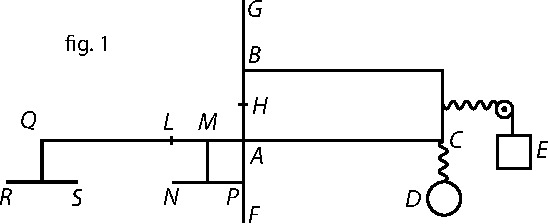
\includegraphics[width=0.58\textwidth]{gesamttex/edit_VIII,3/images/LH_37_03_073-074_d01.pdf}}%\\
\vspace{0.2em}
\centerline{\lbrack\textit{Fig.~1}\rbrack}%
\label{LH_37_03_073r_Fig.1}%
 \vspace{0.9em}
\pstart
\noindent
abrumpenda\protect\index{Sachverzeichnis}{trabs abrumpenda}
opere ponderis \textit{D}\protect\index{Sachverzeichnis}{pondus abrumpens}
applicati ad vectem \textit{AC}:\protect\index{Sachverzeichnis}{vectis}
ubi manifestum est, si vel minimum
\edtext{a muro\protect\index{Sachverzeichnis}{murus perpolitus}}{%
\lemma{a}\Bfootnote{% 
\hspace{-0,5mm}muro \textit{erg.~L}}}
%
\edtext{removeatur \textit{B},
posita rigiditate tabulae,\protect\index{Sachverzeichnis}{rigiditas tabulae}
aerem admitti,\protect\index{Sachverzeichnis}{aer admissus}}{%
\lemma{removeatur \textit{B},}\Bfootnote{%
\textit{(1)}~eti
\textit{(2)}~aditum aeri fi
\textit{(3)}~in fig.
\textit{(4)}~posita rigiditate tabulae,
\textit{(a)}~etiam
\textit{(b)}~aerem admitti,%
~\textit{L}}}
%
et tabulam posse
\edtext{\lbrack separari;\rbrack}{%
\lemma{separi,}\Bfootnote{%
\textit{L~ändert Hrsg.}}}
%
quod si solida\protect\index{Sachverzeichnis}{corpus solidum}
\edtext{quaedam a}{%
\lemma{quaedam}\Bfootnote{%
\textit{(1)}~ex
\textit{(2)}~a%
~\textit{L}}}
%
Tabulis exiguis\protect\index{Sachverzeichnis}{tabula exiguatabulae}
ita sibi invicem applicatis\protect\index{Sachverzeichnis}{tabulae sibi applicatae}
composita intelligamus,
eadem locum habebit % \edlabel{LH_37_03_073r3}
ratiocinatio.\edlabel{LH_37_03_073r_zweiplatten_ndybf-2}\protect\index{Sachverzeichnis}{ratiocinatio}%
% \edtext{}{{\xxref{LH_37_03_073r3}{LH_37_03_073r4}}%
% {\lemma{ratiocinatio.}\Bfootnote{%
% \textit{(1)}~Patet autem
% \textit{(2)}~Patet autem 
% redeundo ad fig.~1 aerem elevationi Tabulae magis resistere in \textit{B}, quam in loco aliquo inter \textit{A} et \textit{B} medio ut \textit{H}, et quidem in ratione \textit{BA} ad \textit{HA}. Continuetur \textit{CA} in \textit{L}, et sit \textit{AL} aequ. \textit{AB}, et
% \textit{(a)}~\textit{AH} ae
% \textit{(b)}~\textit{AM} aequ. \textit{AH} et ita porro in caeteris punctis. Sit \textit{M} centrum gravitatis ipsius \textit{AL} ex quo libere suspendatur \textit{NP} aequalis et similis ipsi \textit{AL} vel \textit{AB}. Continuetur porro \textit{AL} usque in \textit{Q} ut sit \textit{AQ} aequalis ipsi \textit{AC}.
% \textit{(aa)}~Sitque pondus
% \textit{(bb)}~Unde patet si pondus \textit{D} est in ae
% \textit{(cc)}~Unde
% \textit{(aaa)}~eadem
% \textit{(bbb)}~suspendatur \textit{RS} etiam aequalis et similis ipsi \textit{NP} \textbar~vel \textit{AB} \textit{erg.}~\textbar~.
% \textit{(aaaa)}~Patet \textit{CD}
% \textit{(bbbb)}~Sitque \textit{RS} tanti ponderis, quantum est pondus ipsius \textit{E}, erit in aequilibrio cum \textit{E} suspenso ex \textit{C}, at \textit{NP} erit in aequilibrio cum \textit{D} suspenso ex \textit{C}; ergo erit \textit{D} ad \textit{E}, ut \textit{AM} ad \textit{AQ} seu ut \textit{AH} ad \textit{AC}.
% \textit{(3)}~Ut res distinctius%
% ~\textit{L}}}%
% {\lemma{ratiocinatio \lbrack...\rbrack\ distinctius}\Cfootnote{%
% Im gestrichenen Text bezieht sich die Variante \textit{(2)} auf das teilweise gestrichene Diagramm \lbrack\textit{Fig.~1}\rbrack\ auf S.~\pageref{LH_37_03_073r_Fig.1}.}}}
%
\pend%
\vspace{0.5em}%
%
\pstart%
\noindent%
\lbrack\textit{Nachfolgend kleingedruckter Text in L gestrichen:}\rbrack\
\pend%
%
\pstart%
\footnotesize%
Patet\edlabel{LH_37_03_073r_coeiuwvon-1} autem redeundo ad
fig.~1 % \edtext{}{\lemma{fig.~1}\Cfootnote{%
% Das teilweise gestrichene Diagramm \lbrack\textit{Fig.~1}\rbrack\ auf S.~\pageref{LH_37_03_073r_Fig.1}.}}
%
aerem elevationi Tabulae magis resistere in \textit{B},
quam in loco aliquo inter \textit{A} et \textit{B} medio ut \textit{H},
et quidem in ratione \textit{BA} ad \textit{HA}. Continuetur \textit{CA} in \textit{L}, et sit \textit{AL} aequ. \textit{AB}, et
% \textit{(a)}~\textit{AH} ae \textit{(b)}~
\textit{AM} aequ. \textit{AH} et ita porro in caeteris punctis.
Sit \textit{M} centrum gravitatis ipsius \textit{AL}
ex quo libere suspendatur \textit{NP} aequalis et similis ipsi \textit{AL} vel \textit{AB}.
Continuetur porro \textit{AL} usque in \textit{Q}
ut sit \textit{AQ} aequalis ipsi
\edtext{\textit{AC}.
Unde suspendatur \textit{RS} etiam aequalis et similis ipsi \textit{NP}, vel \textit{AB},
sitque \textit{RS} tanti ponderis,
quantum est pondus ipsius \textit{E},
erit in aequilibrio}{%
\lemma{\textit{AC}.}\Bfootnote{%
\textit{(1)}~Sitque pondus
\textit{(2)}~Unde patet, si pondus \textit{D} est in ae
\textit{(3)}~Unde
\textit{(a)}~eadem
\textit{(b)}~suspendatur \textit{RS} \lbrack...\rbrack\ ipsi \textit{NP}, % etiam aequalis et similis
\textbar~vel \textit{AB}, \textit{erg.}~\textbar\
\textit{(aa)}~patet \textit{CD}
\textit{(bb)}~sitque \textit{RS} \lbrack...\rbrack\ in aequilibrio% % tanti ponderis, quantum est pondus ipsius \textit{E}, erit
~\textit{L}}}
%
cum \textit{E} suspenso ex \textit{C},
at \textit{NP} erit in aequilibrio cum \textit{D} suspenso ex \textit{C};
ergo erit \textit{D} ad \textit{E},
ut \textit{AM} ad \textit{AQ} seu ut \textit{AH} ad \textit{AC}.\edlabel{LH_37_03_073r_coeiuwvon-2}%
%
%%    %%    %%    %%    A C H T U N G   G E T R I X T    !!    !!    !!    !!
\edtext{}{%
\lemma{\hspace{1,6mm}\lbrack\textit{Fig.~1}\rbrack}\killnumber\Cfootnote{Der Teil des Diagramms links der Linie \textit{GF} ist gestrichen und auf den gestrichenen Text  bezogen.}}%
\pend%
\vspace{0.8em}
\centerline{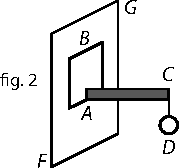
\includegraphics[width=0.22\textwidth]{gesamttex/edit_VIII,3/images/LH_37_03_073-074_d02.pdf}}%\\
\vspace{0.2em}
\centerline{\lbrack\textit{Fig.~2}\rbrack}%
 \label{LH_37_03_073r_Fig.2}%
%%
%%
%\vspace*{2.5em}
%\centerline{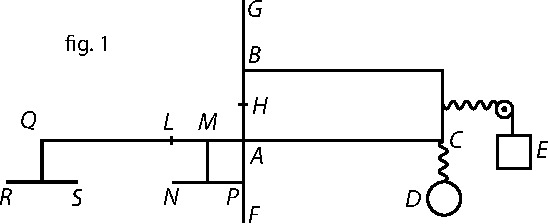
\includegraphics[width=0.60\textwidth]{gesamttex/edit_VIII,3/images/LH_37_03_073-074_d01.pdf}}%\\
%\vspace*{1.0em}
%\centerline{\lbrack\textit{Fig.~1}\rbrack}%
%\label{LH_37_03_073r_Fig.1}%
%% \vspace*{1.5em}
%
%
  \newpage
  \centerline{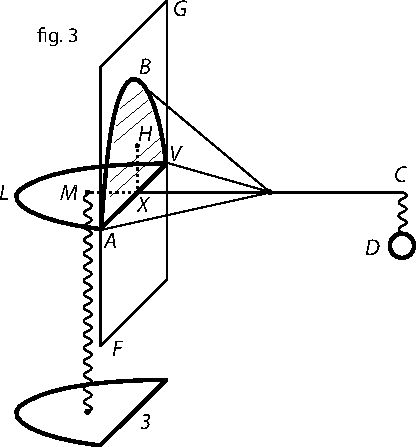
\includegraphics[width=0.48\textwidth]{gesamttex/edit_VIII,3/images/LH_37_03_073-074_d03.pdf}}%\\
  \vspace{0.4em}
  \centerline{\lbrack\textit{Fig.~3}%
  \rbrack\label{LH_37_03_073r_Fig.3}}%
%  \newpage
  \vspace{1.2em}%
%
%
\pstart%
Ut\edlabel{LH_37_03_073r-v_ergebnisse_vubhed-1}
res distinctius appareat,
generaliusque
\edtext{enuntietur
considerabimus totum tabulae planum,\protect\index{Sachverzeichnis}{tabula avellenda}}{%
\lemma{enuntietur}\Bfootnote{%
\textit{(1)}~trabem solidam considerabimus
\textit{(2)}~consideramus
\textit{(3)}~considerabimus totum tabulae planum,%
~\textit{L}}}
%
quod in 
%fig.~3\protect\index{Sachverzeichnis}{figura} %%diese Zeile eingefügt wegen Löschung der CfootnoteKZEITZ
\edtext{fig.~3\protect\index{Sachverzeichnis}{figura}}{%
\lemma{fig.~3}\Cfootnote{%
Das Diagramm \lbrack\textit{Fig.~3}\rbrack\ }}
%%%auskommentiert da Text direkt unter der abbildung stehtKZEITZ
sit \textit{ABV},
\edtext{avellendum a muro\protect\index{Sachverzeichnis}{murus} \textit{FG}
ope vectis \textit{CX}\protect\index{Sachverzeichnis}{vectis}}{%
\lemma{avellendum}\Bfootnote{%
\textit{(1)}~vect
\textit{(2)}~\textbar~avellendum \textit{streicht Hrsg.}~\textbar\ a muro \textit{FG} ope vectis
\textit{(a)}~\textit{CAV}
\textit{(b)}~\textit{CX}%
~\textit{L}}}
%
cui appensum est pondus \textit{D}.\protect\index{Sachverzeichnis}{pondus appensum}
In plano \textit{CAV} continuato ponatur figura \textit{ALV} aequalis et similis ipsi \textit{ABV}
eaque \edtext{figura\protect\index{Sachverzeichnis}{figura aequalis et similis}
sit basis corporis cylindroidis\protect\index{Sachverzeichnis}{corpus cylindroides}
cujus quaelibet sectio horizontalis sit ipsi \textit{ALV} aequalis et similis,
sitque is cylinder\protect\index{Sachverzeichnis}{cylinder}
ejus materiae\protect\index{Sachverzeichnis}{materia} et altitudinis sive crassitiei,}{%
\lemma{figura}\Bfootnote{%
\hspace{-0,5mm}sit
\textit{(1)}~tantae
\textit{(2)}~talis materiae et crassitiei, ita ut instar portionis cylindricae sit
\textit{(3)}~basis
\textit{(a)}~cylindrica ejus materiae et crassitiei
\textit{(b)}~corporis cylindroidis
\textit{(aa)}~quod
\textit{(bb)}~cujus quaelibet \lbrack...\rbrack\ sive crassitiei,%
% sectio horizontalis sit ipsi \textit{ALV} aequalis et similis, sitque is cylinder ejus materiae et altitudinis
~\textit{L}}}
%
ut sit in aequilibrio\protect\index{Sachverzeichnis}{aequilibrium} cum corpore \textit{D},
quod tabulam \textit{ABV}\protect\index{Sachverzeichnis}{tabula avellenda}
a muro\protect\index{Sachverzeichnis}{murus} avellere posse ponamus,
hujus corporis centrum gravitatis sit \textit{M},
ex quo si libere suspendatur corpus \textit{3}%
\protect\index{Sachverzeichnis}{corpus libere suspensum}
ipsi \textit{ALV} cylin\-dri\-co\protect\index{Sachverzeichnis}{corpus cylindricum}
aequale et simile,
id eodem modo erit
\edtext{in}{%
\lemma{in}\Bfootnote{%
\textit{erg.~L}}}
%
aequilibrio\protect\index{Sachverzeichnis}{aequilibrium}
cum pondere \textit{D} suspenso ex \textit{C},\protect\index{Sachverzeichnis}{pondus suspensum}
adeoque erit
\edtext{ad pondus \textit{D}, ut \textit{CX} ad \textit{MX}.}{%
\lemma{ad}\Bfootnote{%
\hspace{-0,5mm}pondus \textit{D},
\textit{(1)}~ut reciproce
\textit{(2)}~ut \textit{CX} ad \textit{MX}.%
~\textit{L}}}
%
Est
\edtext{autem pondus \textit{3} absolute sumtum libereque}{%
\lemma{autem}\Bfootnote{% 
\hspace{-0,5mm}pondus
\textit{(1)}~libere
\textit{(2)}~\textit{3} absolute sumtum libereque%
~\textit{L}}}
%
elevandum ad pondus \textit{D} etiam libere elevandum,
ut resistentia\protect\index{Sachverzeichnis}{resistentia tabulae}
\edtext{Tabulae directe}{%
\lemma{Tabulae}\Bfootnote{%
\textit{(1)}~perpendiculariter
\textit{(2)}~directe%
~\textit{L}}}
%
avellendae ad
\edtext{avellendam circulariter\protect\index{Sachverzeichnis}{tabula avellenda}
per modum vectis.\protect\index{Sachverzeichnis}{vectis}
Ergo haec erit ad illam}{%
\lemma{avellendam}\Bfootnote{%
\textit{(1)}~parallele
\textit{(2)}~circulariter
\textit{(a)}~per modum ve
\textit{(b)}~per modum vectis.
Ergo \textit{(aa)}~illa
\textit{(bb)}~haec erit ad
\textit{(aaa)}~hanc
\textit{(bbb)}~illam%
~\textit{L}}}
%
ut \textit{XH} distantia centri gravitatis\protect\index{Sachverzeichnis}{distantia centri gravitatis}
tabulae\protect\index{Sachverzeichnis}{centri gravitatis tabulae}
a basi \edtext{ejus,
seu horizontali infima \textit{AV}, ad}{%
\lemma{ejus,}\Bfootnote{%
\textit{(1)}~\textit{AV}, ad
\textit{(2)}~seu
\textit{(a)}~minima
\textit{(b)}~horizontali infima \textit{AV}, ad%
~\textit{L}}}
%
\textit{XC} distantiam ponderis.\protect\index{Sachverzeichnis}{distantia ponderis}
% \pend%
%
\lbrack73~v\textsuperscript{o}\rbrack\ % Blatt 73v 
%
%
% \pstart%
Hinc
\edtext{solas lineas\protect\index{Sachverzeichnis}{linea avellenda} considerando}{%
\lemma{solas}\Bfootnote{%
\hspace{-0,5mm}lineas considerando \textit{erg.~L}}}%
\lbrack:\rbrack\
%
si sit linea \textit{AB},
\edtext{fig.~1,\protect\index{Sachverzeichnis}{figura}}{\lemma{fig.~1}\Cfootnote{%
Das Diagramm \lbrack\textit{Fig.~4}\rbrack}}
%
cujus centrum gravitatis \textit{H},
avellenda a muro \textit{FG},\protect\index{Sachverzeichnis}{murus}
erit pondus \textit{E}\protect\index{Sachverzeichnis}{pondus avellens}
\edtext{avellens directe}{%
\lemma{avellens}\Bfootnote{%
\textit{(1)}~parallele
\textit{(2)}~circulariter
\textit{(3)}~directe%
~\textit{L}}}
%
ad pondus \textit{D}\protect\index{Sachverzeichnis}{pondus evellens}
\edtext{evellens circulariter}{%
\lemma{evellens}\Bfootnote{%
\textit{(1)}~perpendiculariter
\textit{(2)}~circulariter%
~\textit{L}}}
%
ope vectis \textit{CA},
\edtext{ut \textit{AH}
(\protect\vphantom)%
altitudo centri gravitatis%
\protect\vphantom()
ad vectem\protect\index{Sachverzeichnis}{vectis}
\lbrack \textit{CA}\rbrack.\edlabel{LH_37_03_073r-v_ergebnisse_vubhed-2}}{%
{\lemma{ut}\Bfootnote{%
\textit{(1)}~vectis
\textit{(2)}~\textit{AH} (\protect\vphantom)altitudo centri gravitatis
\textit{(a)}~seu
\textit{(b)}~\protect\vphantom() ad vectem
\textbar~\textit{CH} \textit{ändert Hrsg.}~\textbar%
~\textit{L}}}%
{\lemma{ut \textit{AH} \lbrack...\rbrack\ vectem \lbrack\textit{CA}\rbrack}\Cfootnote{%
Wie in den Zeilen davor festgestellt, gilt vielmehr die Proportion \textit{E} : \textit{D} = \textit{CA} : \textit{AH}.}}}
%
%
\pend%
%
%
%
\pstart%
Consideremus\edlabel{LH_37_03_073v_TrabsParabolica_hegte-1} jam
\edtext{non pondus vecti}{%
\lemma{non}\Bfootnote{%
\hspace{-0,5mm}pondus
\textit{(1)}~toti
\textit{(2)}~vecti%
~\textit{L}}}
%
appensum,\protect\index{Sachverzeichnis}{pondus vecti appensum}
sed pondus totius
\edtext{vectis,\protect\index{Sachverzeichnis}{pondus vectis} seu}{%
\lemma{vectis,}\Bfootnote{%
\textit{(1)}~et
\textit{(2)}~seu%
~\textit{L}}}
%
Trabis,\protect\index{Sachverzeichnis}{pondus trabis}
et ut ea res cum aliquo fructu fiat,
quaeramus figuram trabis\protect\index{Sachverzeichnis}{figura trabis}
ubique aequaliter resistentis.\protect\index{Sachverzeichnis}{trabs aequiresistens}
\edtext{Fig.~4\protect\index{Sachverzeichnis}{figura}}{%
\lemma{fig.~4}\Cfootnote{%
Das Diagramm \lbrack\textit{Fig.~5}\rbrack}}
%
quaeritur sectio Trabis\protect\index{Sachverzeichnis}{sectio trabis}
prismaticae,\protect\index{Sachverzeichnis}{trabs prismatica}
quae sit \textit{CABDC}
\edtext{figurae}{%
\lemma{figurae}\Bfootnote{%
\textit{erg.~L}}}
%
talis,\protect\index{Sachverzeichnis}{figura trabis}
ut resistentia\protect\index{Sachverzeichnis}{resistentia trabis}
\edtext{ultima in}{%
\lemma{ultima}\Bfootnote{% 
\hspace{-0,5mm}in \textit{erg.~L}}}
%
\textit{AB} sit ad pondus totum\protect\index{Sachverzeichnis}{pondus trabis}
\edtext{\textit{CABDC}, quemadmodum}{%
\lemma{\textit{CABDC},}\Bfootnote{%
\textit{(1)}~ut
\textit{(2)}~quemadmodum%
~\textit{L}}}
%
\edtext{resistentia quaecunque in \textit{DE}
ad pondus\protect\index{Sachverzeichnis}{pondus trabis}
\lbrack quod\rbrack\ ea resistentia\protect\index{Sachverzeichnis}{resistentia trabis}
ferre debet \textit{CEDC}.}{%
\lemma{resistentia}\Bfootnote{%
\textit{(1)}~\textit{CEDC} est
\textit{(2)}~quaecunque in \textit{DE} ad pondus
\textbar~quam \textit{ändert Hrsg.}~%
\textbar\ ea resistentia ferre debet \textit{CEDC}.%
~\textit{L}}}
%
Sit \textit{CE}, \textit{x} et \textit{DE}, \textit{y} et \textit{CA} sit \textit{a}, et \textit{AB}
\edlabel{LH_37_03_073v1}sit \textit{b}.%
%
\edtext{}{%
{\xxref{LH_37_03_073v1}{LH_37_03_073v2}}%
{\lemma{sit}\Bfootnote{% 
\hspace{-0,5mm}\textit{b}.
\textit{(1)}~Utique momentum ipsius \textit{CEDC} ex \textit{EC} est $\displaystyle\!\!\int\!\! y\cdot$
\textit{(2)}~Sic investigabitur
\textit{(3)}~Sit \textit{CK} \textit{z}, et \textit{HK} sit \textit{v}, fiet
\textit{(a)}~$d\overline{v}$
\textit{(b)}~$\displaystyle\!\!\int\!\!\overline{d\overline{z}\,v,\langle\overline{z+v}\rangle}$ ut sit
\textit{(aa)}~$\displaystyle\!\!\int\!\! d\overline{x}$
\textit{(bb)}~$y\,-$
\textit{(4)}~Sit \textit{CK}, \textit{z} et \textit{HK} sit \textit{v},
\textit{(a)}~fiet
\textit{(b)}~et momentum \lbrack...\rbrack\ ex \textit{DE} % ipsius \textit{HK}
\textit{(aa)}~erit: $y\,d\overline{z}$ in $x-z$ ejusque su
\textit{(bb)}~erit \textit{HK} \lbrack...\rbrack\ erit: % in \textit{EK}, seu \textit{vdz} in $x-z.$ Cujus summa 
$\displaystyle\!\!\int\!\!\overline{v \cdot \overline{x-z} \cdot d\overline{z}}.$%
~\textit{L}}}}%
%%    ! ! ! !    A C H T U N G   G E T R I X T    ! ! ! ! 
\edtext{}{\lemma{\lbrack\textit{Fig.~4}\rbrack}\killnumber\Cfootnote{Das Diagramm hieß ursprünglich \textit{fig.~4} und wurde  in \textit{fig.~1} umbenannt.}}
%%
%
%
\pend%
% \vspace*{0.5em}%
% \newpage%
%
%\vspace{2.0em}%
%\centerline{\hspace*{-75mm}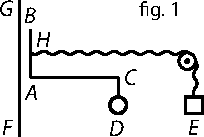
\includegraphics[width=0.24\textwidth]{gesamttex/edit_VIII,3/images/LH_37_03_073-074_d04.pdf}}%
%\vspace{0.5em}
%\centerline{\hspace*{-75mm}\lbrack\textit{Fig.~4}\rbrack}%
%\label{LH_37_03_073v_Fig.4}%
%%
%\vspace*{-9.5em}%
%\centerline{\hspace*{65mm}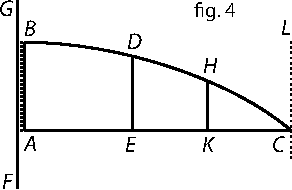
\includegraphics[width=0.34\textwidth]{gesamttex/edit_VIII,3/images/LH_37_03_073-074_d05.pdf}}%
%\vspace*{-1.0em}
%\centerline{\hspace*{65mm}\lbrack\textit{Fig.~5}\rbrack}%
%\label{LH_37_03_073v_Fig.5}%
% \vspace*{2.0em}
 \vspace{1.5em} 
\pstart
\hspace{3mm}
\begin{minipage}[t]{0.5\textwidth}
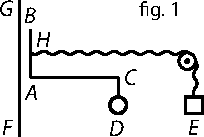
\includegraphics[width=0.46\textwidth]{gesamttex/edit_VIII,3/images/LH_37_03_073-074_d04.pdf}
\end{minipage}
%\hspace{1mm}
\begin{minipage}[t]{0.5\textwidth}
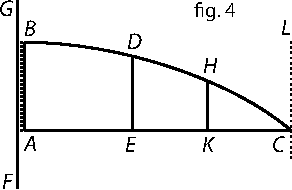
\includegraphics[width=0.67\textwidth]{gesamttex/edit_VIII,3/images/LH_37_03_073-074_d05.pdf}
\end{minipage}
\\
\\\label{LH_37_03_073v_Fig.4}\label{LH_37_03_073v_Fig.5}
\vspace{-0.3em}
\hspace*{19mm} [\textit{Fig.~4}]\hspace*{64mm} [\textit{Fig.~5}]%
\pend
\newpage%
\count\Bfootins=900
\count\Afootins=900
\count\Cfootins=900
\pstart%
\noindent%
\lbrack\textit{Nachfolgend kleingedruckter Text in L gestrichen}:\rbrack\
\pend%
\vspace{0.5em}
%
\pstart%
\noindent%
\footnotesize%
Sit \textit{CK}, \textit{z} et \textit{HK} sit \textit{v},
et momentum ipsius \textit{HK} ex \textit{DE}
erit \textit{HK} in \textit{EK}, seu $v\,d\overline{z}$ in $\overline{x-z}.$%
\protect\index{Sachverzeichnis}{momentum trabis}
Cujus summa\protect\index{Sachverzeichnis}{summa} erit:\protect\rule[-2.5mm]{0mm}{8mm}
$\displaystyle\!\!\int\!\!\overline{v \cdot \overline{x-z} \cdot d\overline{z}}.$%
\edlabel{LH_37_03_073v2}
%
\edtext{Cujus ratio\protect\index{Sachverzeichnis}{ratio ponderis ad resistentiam}
ad resistentiam \textit{ED}\protect\index{Sachverzeichnis}{resistentia trabis}
debet esse constans;\protect\index{Sachverzeichnis}{ratio costans}
\edlabel{LH_37_03_073v_ratioquadratorum_tzoiu-1}ea autem
\edtext{resistentia cum sit in ratione quadratorum \textit{ED}}{%
\lemma{resistentia}\Bfootnote{%
\textit{(1)}~\textit{E}
\textit{(2)}~sit:
\textit{(3)}~cum sit in ratione quadratorum \textit{ED}%
~\textit{L}}}
%
\edlabel{LH_37_03_073v_gekreuzterQuerverweis_rhcg-1}%
ut patet
\edtext{ex supra dictis,%
\edlabel{LH_37_03_073v_gekreuzterQuerverweis_rhcg-2}}{%
\lemma{ex supra dictis}\Cfootnote{%
Siehe vielmehr N.~14\textsubscript{2}, S~\refpassage{LH_37_03_069v_ratioquadratorum-1}{LH_37_03_069v_ratioquadratorum-2}.
Trifft dieser Nachweis zu, so ist der Entwurf N.~14\textsubscript{2} zur gleichen Zeit wie N.~14\textsubscript{1} entstanden und wurde parallel bearbeitet.}}%
\edlabel{LH_37_03_073v_ratioquadratorum_tzoiu-2}
%
ideo faciemus rationem illam talem,
ut sit
$\displaystyle\!\!\int\!\!\overline{v \cdot \overline{x-z} \cdot d\overline{z}}$ aequ. \textit{yyc}
et habebimus:
$v\cdot x-z\cdot dz$ aequ.\protect\rule[-3mm]{0mm}{7mm}
\edtext{$2y\,dy\,c.$
Sed $\displaystyle y\,d\overline{x}$ in}{%
\lemma{$2y\,dy\,c.$}\Bfootnote{%
\textit{(1)}~Seu $x-z\cdot dz$ aequ. \textit{dvc}. cumque sit \textit{dx} aequ. \textit{dz}. fiet $xdx-zdz$ aequ. \textit{cdv}.
\textit{(2)}~Sed
\textit{(a)}~\textit{cc}
\textit{(b)}~$\displaystyle\!\!\int\!\!$
\textit{(c)}~$\displaystyle y\,d\overline{x}$ in %
~\textit{L}}}%
}{%
\lemma{\textit{Am Rand:}}%
\Afootnote{NB. NB. voicy un calcul estrange,
et considerable\protect\index{Sachverzeichnis}{calcul considerable}
quoyqu' il soit effacé\\
\vspace{-0.32em}%
}}
%
\normalsize%
\lbrack\textit{Text bricht ab.}\rbrack%
\pend%
%
\pstart%
\footnotesize%
\textit{CK}, \textit{z}. et \textit{HK}, \textit{v}.
fiet:
$\displaystyle\!\!\int\!\!\overline{v\,d\overline{x}\,\text{in}\,\overline{x-z}}$ aequ. \textit{cyy}
seu
$2cy\,d\overline{y}$ aequ. $v\,d\overline{x}$ in $\overline{x-z}.$
\edtext{%
Quod cum de quovis casu\protect\index{Sachverzeichnis}{casus} sit verum,
erit et verum cum \textit{v} et \textit{z} sunt quantitates determinatae,
\edtext{quod supponere possumus,
quia desunt earum differentiae.
Nam pro differentia ipsius \textit{z} adhibuimus differentiam ipsius \textit{x}
quam posuimus esse constantem,}{% 
\lemma{quod}\Bfootnote{%
\hspace{-0,5mm}supponere \lbrack...\rbrack\ esse constantem,
\textit{erg.~L}}}
ac proinde, fiet:
$2cy\,d\overline{y}$ aequ. $l\,d\overline{x}$ in $\overline{x-m},$
posito relationem\protect\index{Sachverzeichnis}{relatio}
inter \textit{l} et \textit{m} eandem esse
quae est inter \textit{x} et \textit{y}.
Quo facto\protect\rule[-1.5mm]{0mm}{6mm}
\edtext{fiet: \textit{cyy}}{%
\lemma{fiet:}\Bfootnote{%
\textit{(1)}~$2cy\,d$
\textit{(2)}~\textit{cyy}%
~\textit{L}}}
%
aequ. $\displaystyle\frac{1}{2}lxx-lmx$
et posito nos posse alicubi in hac curva\protect\index{Sachverzeichnis}{curva}
sumere \textit{l} et \textit{m} aequales, ordinatam et abscissam,
fiet:%
\protect\rule[0mm]{0pt}{2mm}
\textit{cyy} aequ. $\displaystyle\frac{1}{2}lxx-llx.$
}{%
\lemma{\textit{Am Rand:}}%
\Afootnote{subtilissime\\
\vspace{-0.44em}%
}}%
Ergo et cum \textit{a} sit aliqua ex ipsis \textit{x} et \textit{b} aliqua ex ipsis \textit{y},
fiet:
\textit{cbb} aequ. $\displaystyle\frac{1}{2}laa-lla.$ 
Cumque datae sint \textit{a} et \textit{b}
hinc dabitur etiam relatio\protect\index{Sachverzeichnis}{relatio} inter \textit{c} et \textit{l}.
Datur autem \textit{c} si data sit quantitas resistentiae,
seu ratio ponderis ad\protect\index{Sachverzeichnis}{ratio ponderis ad resistentiam}
\edtext{resistentiam v.g.}{%
\lemma{resistentiam}\Bfootnote{%
\textit{(1)}~posito
\textit{(2)}~v.g.%
~\textit{L}}}
%
potest esse dupla,
si pondus\protect\index{Sachverzeichnis}{pondus trabis} duplicandum sit,
ut vincatur;
itaque data quantitate resistentiae\protect\index{Sachverzeichnis}{resistentia trabis} ubique aequalis,
dataque longitudine\protect\index{Sachverzeichnis}{longitudo trabis}
et altitudine trabis\protect\index{Sachverzeichnis}{altitudo trabis}
datur et ipsa \textit{l} quae
\edtext{sit parameter\protect\index{Sachverzeichnis}{parameter}
\lbrack alicujus\rbrack\
curvae naturae,\protect\index{Sachverzeichnis}{natura curvae}
ut ibi ordinata}{%
\lemma{sit}\Bfootnote{%
\textit{(1)}~latus rectum curvae, seu
\textit{(2)}~parameter \textbar~aliqua \textit{ändert Hrsg.}~\textbar\ curvae
\textit{(a)}~, ejus sc
\textit{(b)}~quae
\textit{(c)}~naturae, ut ibi
\textit{(aa)}~latus rec
\textit{(bb)}~ordinata%
~\textit{L}}}
%
et abscissa sint aequales.%
\edtext{}{%
\lemma{\textit{Am Rand, gestrichen:}}%
\Afootnote{{\footnotesize%
Sit \textit{x}
aequ $z^l$\textsuperscript{[a]} etc.[,] $d\overline{x}$
aequ. $l\cdot z^{l-1}$[,]\textsuperscript{[b]} $d\overline{x}^2$
aequ. $ll\cdot z^{2l-2}$[,]\textsuperscript{[c]} $\displaystyle\!\!\int\!\!d\overline{x}^2$
aequ. $\displaystyle\frac{ll}{2l+2}z^{2l-1}$\\
\vspace{-1mm}
\newline
%
%
\textsuperscript{[a]}\,%
aequ. $z^l$ \textit{(1)}~$+\, z^m$ \textit{(2)}~etc.~\textit{L}%
\quad\quad\quad%
%
\textsuperscript{[b]}\,%
aequ. $l\cdot z^{l-1}$ \textit{(1)}~$+\, mz^{m-1}$ \textit{(2)}~$d\overline{x}^2$~\textit{L}%
\quad\quad\quad%
%
\textsuperscript{[c]}\,%
aequ. $ll\cdot z^{2l-2}$
\textit{(1)}~$+\, 2lm\, z^{l+m-2}+mmz^{2m-2}$ \textit{(2)}~$\displaystyle\!\!\int\!\!d\overline{x}^2$ aequ. \textit{(3)}~$\displaystyle\!\!\int\!\!d\overline{x}^2$ aequ.~\textit{L}\vspace{-6mm}}}}
%
Sit
\edtext{\textit{AB} seu \textit{b}, $1,$}{%
\lemma{\textit{AB}}\Bfootnote{%
\hspace{-0,5mm}\textbar~seu \textit{erg.}~\textbar\ \textit{b}. $1.$%
~\textit{L}}}
%
et \textit{AC} seu \textit{a} sit 3, et \textit{c} sit 2,
fiet:
2 aequ. $\displaystyle\frac{9}{2}l-3ll$
\pend%%%%%%%%%%%%%%%%künstlicher Seitenumbruch mitten im Absatz KZEITZ
\newpage
\count\Bfootins=1100
\count\Afootins=1100
\count\Cfootins=1100
\pstart
\noindent
\footnotesize
seu 4 aequ. $9l-6ll.$
Unde habetur \textit{l}.
Unde etiam deprehendi potest
an suppositiones\protect\index{Sachverzeichnis}{suppositio} sint possibiles,
quando scilicet aequatio nostra est possibilis.\protect\index{Sachverzeichnis}{aequatio possibilis}
Memorabilissima est haec Methodus,\protect\index{Sachverzeichnis}{methodus memorabilis}
quia nondum memini tale exemplum\protect\index{Sachverzeichnis}{exemplum} mihi occurrisse.
Exitum\protect\index{Sachverzeichnis}{exitus} etiam non reperiret,
nisi posuimus $d\overline{x}$ constantem.
Curva\protect\index{Sachverzeichnis}{curva} ergo est parabola.\protect\index{Sachverzeichnis}{parabola}
Sumamus $c.\ b.\ a$ tales ut \textit{l} fiat rationalis,%
\rule[0mm]{0pt}{5mm}
nimirum
$ll-\displaystyle\frac{1}{2}la+\displaystyle\frac{aa}{16}$ aequ. $\displaystyle\frac{aa}{16}-\displaystyle\frac{cbb}{a}$
seu
$\pleibdashv l\ \pleibvdash\displaystyle\!\frac{1}{4}a$ aequ.
\edtext{$\displaystyle\frac{1}{a}\sqrt{a^4-16cabb}$}{%
\lemma{$\displaystyle\frac{1}{a}\sqrt{a^4-16cabb}$}\Cfootnote{%
Der richtige Term ist $\displaystyle\frac{1}{4a}\sqrt{a^4-16ab^2c}.$
Der Fehler wirkt sich auf die folgende Ableitung aus.}}
%
seu
\textit{l} aequ. $\pleibdashv\displaystyle\frac{1}{a}\sqrt{a^4-16acbb}+\displaystyle\frac{1}{4}a.$
%
\pend%
\vspace{0.5em}%
% \newpage%
%
\pstart%
Momentum\protect\index{Sachverzeichnis}{momentum trabis}%
\edlabel{LH_37_03_073v_calculus-1}%
\edlabel{LH_37_03_073v_integralfaktor_ewj-1}
ipsius \textit{CEDC} ex \textit{CL} est
$\displaystyle\!\!\int\!\!\overline{yx\,d\overline{x}}.$%
\edlabel{LH_37_03_073v_integralfaktor_ewj-2}
Quod, si a cylindro\protect\index{Sachverzeichnis}{cylinder} cujus basis \mbox{\textit{CEDC}}, altitudo \textit{CE},
\rule[0mm]{0pt}{5mm}%
detrahatur, seu ab
$\displaystyle x\!\!\int\!\!\overline{y\,d\overline{x}},$
habebitur momentum ex \textit{DE},\protect\index{Sachverzeichnis}{momentum trabis}
quod erit:
$\displaystyle x\!\!\int\!\!\overline{y\,d\overline{x}\ }$%
\edtext{$\displaystyle -\!\!\int\!\!\overline{yx\,d\overline{x}}$ \lbrack et\rbrack\ debet esse aequal.}{%
\lemma{$\displaystyle -\!\!\int\!\!\overline{yx\,d\overline{x}}$}\Bfootnote{%
\hspace{-0,5mm}\textbar~et \textit{erg. Hrsg.}~\textbar\
\textit{(1)}~aequ.
\textit{(2)}~debet esse aequal.%
~\textit{L}}}
%
\textit{cyy}.
\rule[0mm]{0pt}{5mm}%
Unde fiet:
$\displaystyle \ovalbox{$\displaystyle xy\,d\overline{x}$}\, + \!\!\int\!\!\overline{y\, d\overline{x}}\,d\overline{x}\;\ovalbox{$\displaystyle \!-\ yx\,d\overline{x}$}$
\mbox{aequ.}
$2cy\,d\overline{y}$
seu
$\displaystyle \!\!\int\!\!\overline{y\,d\overline{x}}\,d\overline{x}$
\edlabel{LH_37_03_073v7}aequ. $2cy\,d\overline{y}.$%
\edtext{}{{\xxref{LH_37_03_073v7}{LH_37_03_073v8}}%
\lemma{aequ.}\Bfootnote{%
\hspace{-0,5mm}$2cy\,d\overline{y}.$
\textit{(1)}~seu $\displaystyle y\,d\overline{x}d\overline{x}\, + \!\!\int\!\!\overline{y\,d\overline{x}}\ \overline{d\overline{d\overline{x}}}$ aequ. $2c\,d\overline{y}d\overline{y}+2cy\,d\overline{d\overline{y}}.$ $d\overline{x}$ vocemus \textit{z} et $d\overline{y}$ vocemus \textit{v}, fiet:  \textit{zz} aequ. $\displaystyle\frac{2cvv}{\int\!\!v}+2d\overline{v}$ faciendo $d\overline{d\overline{x}}$ aequ. $0$ fiet: $d\overline{x}^2$ aequ. $2c\,d\overline{y}^2 + 2c\,d\overline{d\overline{y}}$ 
\textit{(2)}~Ponatur \textit{y} aequ. $nx^{\protect\underline{h}}$
\textit{(a)}~\textbar~fiet: \textit{streicht Hrsg.}~\textbar\ $\displaystyle\!\!\int\!\!x^hdx$
\textit{(b)}~erit $d\overline{y}$ aequ. $nhx^{\protect\underline{h-1}}d\overline{x}$
\textit{(aa)}~et fiet
\textit{(bb)}~et $\displaystyle\!\!\int\!\!y\,d\overline{x}$
\textit{(aaa)}~erit
\textit{(bbb)}~seu
\textbar~erit \textit{erg. u. gestr.}~%
\textbar\ $\displaystyle\!\!\int\!\!nx^{\protect\underline{h}}d\overline{x}$ erit:%
~\textit{L}}}
%
\rule[0mm]{0pt}{5mm}%
Ponatur \textit{y} aequ. $nx^{\underline{h}}$
erit
$d\overline{y}$ aequ. $nhx^{\underline{h-1}}d\overline{x}$
et
$\displaystyle\!\!\int\!\!\overline{y\,d\overline{x}}$
seu
$\displaystyle\!\!\int\!\!\overline{nx^{\underline{h}}d\overline{x}}$
erit:\edlabel{LH_37_03_073v8}
\rule[0mm]{0pt}{5mm}%
$\displaystyle\frac{n}{h}x^{\underline{h+1}}.$
Ergo pro aequatione differentiali:\protect\index{Sachverzeichnis}{aequatio differentialis}
$\displaystyle\!\!\int\!\!\overline{y\,d\overline{x}}\,d\overline{x}$ aequ. $2cydy$
fiet: \rule[0mm]{0pt}{5mm}%
$\displaystyle\frac{n}{h}x^{h+1}d\overline{x}$ aequ. $2cnx^{\underline{h}}\cdot nh\cdot x^{\underline{h-1}}d\overline{x}$
seu
$\displaystyle\frac{1}{h}x^{\underline{h+1}}$ aequ. $2cnhx^{\underline{2h-1}},$
et debet esse:
$x^{\underline{h+1}}$ aequ. $x^{\underline{2h-1}}$ seu $h+1$ aequ. $2h-1.$
Fiet \textit{h} aequ. 2.
\protect\rule[-2mm]{0mm}{6mm}Habemus ergo \textit{y} aequ. $nx^2.$
Est autem $\displaystyle\frac{1}{h}$ aequ. $2cnh,$
seu
\edtext{$\displaystyle\langle\frac{1}{h}\rangle$ aequ. $\displaystyle\frac{2cn}{h}$}{%
\lemma{$\displaystyle\langle\frac{1}{h}\rangle$ aequ. $\displaystyle\frac{2cn}{h}$}\Cfootnote{%
Die richtige Gleichung ist $\displaystyle\frac{1}{h^2}=2cn.$
Der Fehler wirkt sich auf die folgenden Ableitungen aus.}}
%
seu \textit{n} aequ. $\displaystyle\frac{1}{2c}.$
Ergo
\edtext{\textlangle eri\textrangle t $2cy$}{%
\lemma{\textlangle eri\textrangle t}\Bfootnote{%
\textit{(1)}~\textit{y} aequ.
\textit{(2)}~$2cy$%
~\textit{L}}}
%
aequ. $x^2$
quae \textlangle est\textrangle\ curva quaesita,\protect\index{Sachverzeichnis}{curva quaesita}
\rule[0mm]{0pt}{5mm}%
nempe
\edlabel{LH_37_03_073v_Umbruch-1}%
parabola.\protect\index{Sachverzeichnis}{parabola}%
\edlabel{LH_37_03_073v_calculus-2}%
\edlabel{LH_37_03_073v_TrabsParabolica_hegte-2}%
%
\edtext{}{{\xxref{LH_37_03_073v_Umbruch-1}{LH_37_03_074r_Umbruch-2}}%
\lemma{parabola.}\Bfootnote{%
\textit{(1)}~Potentiam\protect\index{Sachverzeichnis}{potentia} tamen fortasse pluribus aliis curvis satisface
\lbrack74~r\textsuperscript{o}\rbrack\
\textit{(2)}~Veniamus nunc ad
~\textit{L}}}
%
\lbrack74~r\textsuperscript{o}\rbrack\ %  Blatt 74r%
%
\pend%
% \vspace*{0.5em}%
\newpage%
%
\pstart%
\noindent%
\lbrack\textit{Nachfolgend kleingedruckter Text in L gestrichen}:\rbrack\
\pend%
\vspace{0.5em}%
%
\pstart%
\footnotesize%
Veniamus nunc ad\edlabel{LH_37_03_074r_Umbruch-2}
alteram Hypothesin\protect\index{Sachverzeichnis}{hypothesis altera}
qua supponitur solidum esse tensile.%
\protect\index{Sachverzeichnis}{solidum tensile}\protect\index{Sachverzeichnis}{corpus trabis tensile}
Ponamus
\edtext{fig.~5\protect\index{Sachverzeichnis}{figura}}{%
{\lemma{fig.~5}\Bfootnote{%
\textit{erg.~L}}}%
{\lemma{fig.~5}\Cfootnote{%
Das Diagramm \lbrack\textit{Fig.~6}\rbrack\ auf S.~\pageref{LH_37_03_074r_Fig.6}.??}}}
%
lineam \textit{AB} funiculis\protect\index{Sachverzeichnis}{funiculus}
annexam parieti\protect\index{Sachverzeichnis}{paries} \textit{FG},
eosque funes esse aequaliter fortes et tensos,\protect\index{Sachverzeichnis}{funis tensus}
ut determinata vi eadem unusquisque eorum rumpi possit.\protect\index{Sachverzeichnis}{vis rumpens}
\edtext{Patet tensionem funis\protect\index{Sachverzeichnis}{tensio funis}}{%
\lemma{Patet}\Bfootnote{%
\textit{(1)}~funem
\textit{(2)}~tensionem funis%
~\textit{L}}}
%
\textit{B} esse ad tensionem funis \textit{H},
in ratione \textit{AB} ad \textit{AH}.
\edtext{Et funem \textit{B} rumpi}{%
\lemma{Et}\Bfootnote{%
\textit{(1)}~rumpi
\textit{(2)}~corpus \textit{AB} abrumpi
\textit{(3)}~funem \textit{B} rumpi%
~\textit{L}}}
%
ubi ad summam tensionem\protect\index{Sachverzeichnis}{tensio funis}
quam ferre potest pervenerit,
rupto autem fune \textit{B},\protect\index{Sachverzeichnis}{funis tensus}
continuanteque nisu ponderis \textit{D},\protect\index{Sachverzeichnis}{nisus ponderis}
statim mox et inferior rumpetur \textit{K},
et rupto \textit{K} statim proximus \textit{H},
et ita porro, et
\edtext{proinde totum}{%
\lemma{proinde}\Bfootnote{%
\textit{(1)}~totus
\textit{(2)}~totum%
~\textit{L}}}
%
abrumpetur.\protect\index{Sachverzeichnis}{ruptura funis}
Quod si lineam \textit{AHKB} ponamus esse rectam,
aestimari potest vis ad rumpendum necessaria.\protect\index{Sachverzeichnis}{vis ad rumpendum necessaria}
Nam ubi tensio ipsius \textit{B}\protect\index{Sachverzeichnis}{tensio funis}
erit maxima quam ferre potest,\protect\index{Sachverzeichnis}{tensio maxima}
rumpetur,\protect\index{Sachverzeichnis}{ruptura funis}
erit
\edtext{autem talis,
ubi}{%
\lemma{autem}\Bfootnote{%
\textit{(1)}~, ubi
\textit{(2)}~talis, ubi%
~\textit{L}}}
%
vis tendens\protect\index{Sachverzeichnis}{vis tendens} erit aequalis aggregato omnium
\edtext{tensionum.\protect\index{Sachverzeichnis}{aggregatum tensionum}
Sit Tensio maxima\protect\index{Sachverzeichnis}{tensio maxima}}{%
\lemma{tensionum}\Bfootnote{%
\textit{(1)}~, id est dimidio
\textit{(2)}~. Sit Tensio maxima%
~\textit{L}}}
%
quam ferre aliquis locus, ut \textit{B}, potest, \textit{t},
ducta in
\edtext{\lbrack\textit{AB}\rbrack}{%
\lemma{\textit{AQ}}\Bfootnote{%
\textit{L~ändert \mbox{Hrsg.}}}}
%
seu \textit{a},
erit \textit{at} vis quae perpendiculariter rumpere potest,\protect\index{Sachverzeichnis}{vis rumpendi}
seu vis in singulis punctis ducta in longitudinem seu aggregatum omnium punctorum\lbrack,\rbrack\
sed vis quae rumpere potest parallele aequatur
\edtext{tensionibus quae sunt ut}{%
\lemma{tensionibus}\Bfootnote{%
\textit{(1)}~ipsius
\textit{(2)}~quae sunt ut%
~\textit{L}}}
%
rectae \textit{B}. \textit{K}. \textit{H} etc.
Quarum summa est dimidium summae\protect\index{Sachverzeichnis}{summa tensionum}
\edlabel{LH_37_03_074r_Umbruch-3}prioris.%
%
\edtext{}{%
{\xxref{LH_37_03_074r_Umbruch-3}{LH_37_03_074r_Umbruch-4}}
{\lemma{prioris.}\Bfootnote{%
\textit{(1)}~Video
\textit{(2)}~Veniamus nunc ad%
~\textit{L}}}}
\pend%
%
%
%  \newpage
  \vspace{1.5em}%
  \centerline{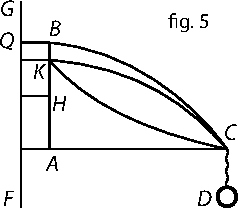
\includegraphics[width=0.24\textwidth]{gesamttex/edit_VIII,3/images/LH_37_03_073-074_d06.pdf}}% \hspace{-70mm}
  \vspace{0.5em}
  \centerline{\lbrack\textit{Fig.~6, gestr.}\rbrack}\label{LH_37_03_074r_Fig.6}%
  \vspace{1.5em}
%
%
\pstart%
Veniamus\edlabel{LH_37_03_074r_zweiterTeil_lbhuno-1}
nunc ad\edlabel{LH_37_03_074r_Umbruch-4}
alteram Hypothesin,\protect\index{Sachverzeichnis}{hypothesis altera}
qua solidum consideratur ut tensile.%
\protect\index{Sachverzeichnis}{solidum tensile}\protect\index{Sachverzeichnis}{corpus trabis tensile}
\edtext{Sit paries\protect\index{Sachverzeichnis}{paries}}{%
\lemma{Sit}\Bfootnote{%
\textit{(1)}~murus
\textit{(2)}~paries%
~\textit{L}}}%
\edtext{ \textit{FG},}{%
\lemma{paries \textit{FG}}\Cfootnote{Siehe \lbrack\textit{Fig.~7}\rbrack\ auf S.~\pageref{LH_37_03_074r_Fig.7}.??}}
%
ex quo prodeat sustentaculum \textit{H},\protect\index{Sachverzeichnis}{sustentaculum}
in
\edtext{quo infixa rotula \textit{A},\protect\index{Sachverzeichnis}{rotula}
sic tamen ut circa suum axem\protect\index{Sachverzeichnis}{axis} moveri possit}{%
\lemma{quo}\Bfootnote{%
\textit{(1)}~mobiliter
\textit{(2)}~infixa rotula \lbrack...\rbrack\ moveri possit%
~\textit{L}}}
%
et cum ea infixus rotulae\protect\index{Sachverzeichnis}{rotula}
angulus rectus \textit{BAC}.\protect\index{Sachverzeichnis}{angulus rectus mobilis}
Ponamus \textit{AB} et \textit{AC} esse aequales,
et latus \textit{AB} esse
\edtext{erectum verticaliter seu}{%
\lemma{erectum}\Bfootnote{%
\textit{(1)}~seu
\textit{(2)}~verticaliter seu%
~\textit{L}}}
%
parieti\protect\index{Sachverzeichnis}{paries} parallelum,
eique alligatum chordis aequalibus et
\edtext{similibus}{%
\lemma{similibus,}\Bfootnote{%
\textit{erg.~L}}}
%
aequaliter\protect\index{Sachverzeichnis}{chorda tensa}
\edtext{tensis horizonti parallelis \textit{IK},}{%
\lemma{tensis}\Bfootnote{%
\textit{(1)}~quotcunque \textit{IK}, paral
\textit{(2)}~horizonti parallelis \textit{IK},%
~\textit{L}}}
%
\textit{LM}, \textit{NO}, \textit{BQ} aliisque quotcunque
\edtext{intermediis,
tensae autem sunt hae chordae,\protect\index{Sachverzeichnis}{chorda tensa}}{%
\lemma{intermediis,}\Bfootnote{%
\textit{(1)}~et in \textit{C} alligatum sit pondus \textit{D} quod chordas nisu suo tendit
\textit{(2)}~tensae autem sunt hae chordae,%
~\textit{L}}}
%
quia obstaculum\protect\index{Sachverzeichnis}{obstaculum} \textit{rI} prohibet
quominus \textit{AB} possit ad murum\protect\index{Sachverzeichnis}{murus} accedere.
Ponamus
\edtext{jam \lbrack datum\rbrack\ esse pondus~\textit{E}\protect\index{Sachverzeichnis}{pondus avellens}
quod \textit{AB} avellere possit a pariete\protect\index{Sachverzeichnis}{paries}
directe\protect\index{Sachverzeichnis}{pondus directe tendens}
seu directione \textit{st} perpendiculari ad murum,\protect\index{Sachverzeichnis}{murus}
quaeritur pondus \textit{D}\protect\index{Sachverzeichnis}{pondus circulariter tendens}
quod conatu circulari\protect\index{Sachverzeichnis}{conatus circularis} ex centro \textit{A},
vecte \textit{AC}\protect\index{Sachverzeichnis}{vectis} avellere possit idem corpus \textit{AB}.
Quod ut aestimetur\lbrack,\rbrack\
tensio chordarum\protect\index{Sachverzeichnis}{tensio chordae} consideranda est.
Sint in\protect\index{Sachverzeichnis}{figura}
\edtext{fig.~6}{\lemma{fig.~6}\Cfootnote{Das Diagramm \lbrack\textit{Fig.~8}\rbrack\ auf S.~\pageref{LH_37_03_074r_Fig.8}.??}}%
}{% 
\lemma{jam}\Bfootnote{%
\hspace{-0,5mm}\textbar~datam \textit{ändert Hrsg.}~\textbar\ esse
\textit{(1)}~vim
\textit{(a)}~quae pondus nimirum
\textit{(b)}~quae
\textit{(2)}~pondus qu
\textit{(3)}~pondus \textit{E}
\textit{(a)}~quod
\textit{(b)}~quod \textit{AB} \textbar~avellere possit \textit{erg.}~\textbar\ a
\textit{(aa)}~muro
\textit{(bb)}~pariete directe
\textit{(aaa)}~nisuque ad
\textit{(bbb)}~seu directione
\textit{(aaaa)}~pe
\textit{(bbbb)}~per
\textit{(cccc)}~\textit{st}
\textit{(dddd)}~\textbar~\textit{st} \textit{erg.}~\textbar\ perpendiculari ad murum,
\textit{(aaaaa)}~\textit{st}
\textit{(bbbbb)}~seu pondus
\textit{(ccccc)}~quaeritur pondus \textit{D} quod
\textit{(aaaaa-a)}~nisu ad murum parallelo
\textit{(bbbbb-b)}~conatu circulari \lbrack...\rbrack\ vecte \textit{AC} % ex centro \textit{A},
\textit{(aaaaa-aa)}~ipsam
\textit{(bbbbb-bb)}~avellere possit idem corpus \textit{AB}.
\textit{(aaaaa-aaa)}~Quod ut aestimetur considerandum est primo
\textit{(bbbbb-bbb)}~Quod ut \lbrack...\rbrack\ fig.~6.%
~\textit{L}}}
%
duae chordae \textit{ae} et \textit{cf}\protect\index{Sachverzeichnis}{chorda tensa}
% \edtext{}{%
% \lemma{chordae}\Bfootnote{%
% \textit{(1)}~simil
% \textit{(2)}~\textit{ae} et \textit{cf}%
% ~\textit{L}}}
%
per omnia similes et
\edtext{aequales si sibi relinquantur.
Quarum una appenso pondere\protect\index{Sachverzeichnis}{pondus appensum}}{%
\lemma{aequales}\Bfootnote{%
\textit{(1)}~quarum una appenso pondere
\textit{(2)}~si sibi \lbrack...\rbrack\ appenso pondere%
~\textit{L}}}
%
\textit{b} extensa sit\protect\index{Sachverzeichnis}{chorda extensa}
\edtext{ex \textit{ae}}{%
\lemma{ex}\Bfootnote{%
\hspace{-0,5mm}\textit{ae}
\textit{erg.~L}}}
%
in\hfill \textit{ab},\hfill
altera\hfill appenso\hfill pondere\hfill \textit{d}\hfill extensa\protect\index{Sachverzeichnis}{chorda extensa}
\edtext{ex \textit{cf}}{%
\lemma{ex}\Bfootnote{%
\hspace{-0,5mm}\textit{cf}
\textit{erg.~L}}} \hspace{0.2mm}usque\hspace{0.2mm} in \textit{cd}.
%
%
\pend
\vspace{2.0em}
\count\Bfootins=1000
\count\Afootins=1000
\count\Cfootins=1000
%%
%%
%\newpage
%%  \vspace*{0.0em}%
%%  \centerline{\hspace{-70mm}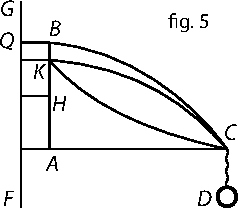
\includegraphics[width=0.25\textwidth]{gesamttex/edit_VIII,3/images/LH_37_03_073-074_d06.pdf}}%
%%  \vspace*{0.5em}
%%  \centerline{\hspace{-70mm}\lbrack\textit{Fig.~6, zu gestrichenem Text}\rbrack}\label{LH_37_03_074r_Fig.6}%
%%\vspace*{0.0em}%
%  \centerline{\hspace{-80mm}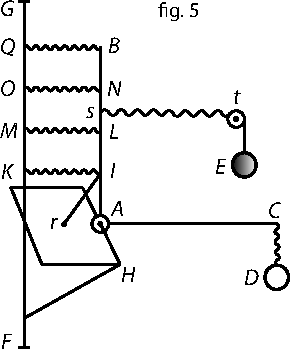
\includegraphics[width=0.36\textwidth]{gesamttex/edit_VIII,3/images/LH_37_03_073-074_d07.pdf}}%
%  \vspace{-1.5em}
%  \centerline{\hspace{-74mm}\lbrack\textit{Fig.~7}\rbrack}\label{LH_37_03_074r_Fig.7}%
%%  \edtext{}{\lemma{\lbrack\textit{Fig.~7}\rbrack}\killnumber\Cfootnote{**************************}}
%%
%  \vspace{-17.0em}%
%  \centerline{\hspace{30mm}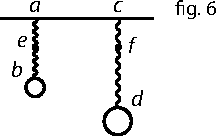
\includegraphics[width=0.26\textwidth]{gesamttex/edit_VIII,3/images/LH_37_03_073-074_d08.pdf}}%
%  \vspace{-0.5em}
%  \centerline{\hspace{7mm}\lbrack\textit{Fig.~8}\rbrack}\label{LH_37_03_074r_Fig.8}%  
%%  \edtext{}{\lemma{\lbrack\textit{Fig.~8}\rbrack}\killnumber\Cfootnote{**************************}}
%%  \newpage
%%
%  \vspace{11.0em}%
%  \centerline{\hspace{-1mm}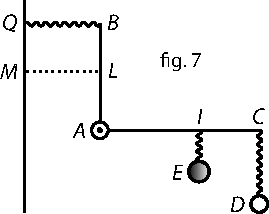
\includegraphics[width=0.34\textwidth]{gesamttex/edit_VIII,3/images/LH_37_03_073-074_d09.pdf}}%
%  \vspace{-1.0em}
%  \centerline{\hspace{-4mm}\lbrack\textit{Fig.~9}\rbrack}\label{LH_37_03_074r_Fig.9}%  
%%  \edtext{}{\lemma{\lbrack\textit{Fig.~9}\rbrack}\killnumber\Cfootnote{**************************}}
%%
%  \vspace*{-22.0em}%
%  \centerline{\hspace{90mm}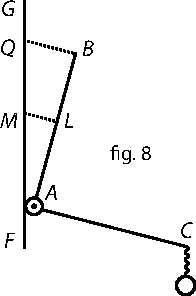
\includegraphics[width=0.24\textwidth]{gesamttex/edit_VIII,3/images/LH_37_03_073-074_d10.pdf}}%
%  \vspace*{-1.5em}
%  \centerline{\hspace{90mm}\lbrack\textit{Fig.~10}\rbrack}\label{LH_37_03_074r_Fig.10}%
%%  \edtext{}{\lemma{\lbrack\textit{Fig.~10}\rbrack}\killnumber\Cfootnote{**************************}}
%  \vspace*{10.0em}%
  %%%%%%%%%%%%%%%%%%%%%%%%%%%%%%%%%%%%%%%%%%%%%%%%%%%%%%%%%%%%%%%%%%
% \newpage%
   \centerline{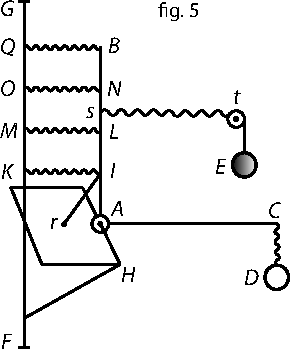
\includegraphics[width=0.33\textwidth]{gesamttex/edit_VIII,3/images/LH_37_03_073-074_d07.pdf}}%
  \vspace{0.5em}
  \centerline{\lbrack\textit{Fig.~7}\rbrack}\label{LH_37_03_074r_Fig.7}%
  %\vspace{1em}
  \newpage
  \pstart  \noindent
\begin{minipage}[t]{0.33\textwidth}
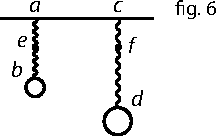
\includegraphics[width=0.74\textwidth]{gesamttex/edit_VIII,3/images/LH_37_03_073-074_d08.pdf}
\end{minipage}
%\hspace*{13,3mm}
\begin{minipage}[t]{0.33\textwidth}
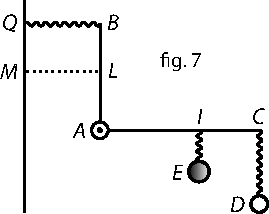
\includegraphics[width=0.92\textwidth]{gesamttex/edit_VIII,3/images/LH_37_03_073-074_d09.pdf}
\end{minipage}
\hspace{11mm}
\begin{minipage}[t]{0.33\textwidth}
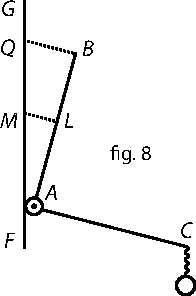
\includegraphics[width=0.69\textwidth]{gesamttex/edit_VIII,3/images/LH_37_03_073-074_d10.pdf}
\end{minipage}
\\
\\
\hspace*{10mm} [\textit{Fig.~8}]\label{LH_37_03_074r_Fig.8}\hspace*{39mm} [\textit{Fig.~9}]\label{LH_37_03_074r_Fig.9}\hspace*{35mm} [\textit{Fig.~10}]\label{LH_37_03_074r_Fig.10}
\pend
\vspace{2.5em}
%%%%%%%%%%%%%%%%%%%%%%%%%%%%%%%%%%%%%%%%%%%%%%%%%%%%%%%%%%%%%%%%%%%%%
\pstart
\noindent
Erunt\setline{1} vires\protect\index{Sachverzeichnis}{vis tendens}
seu pondera\protect\index{Sachverzeichnis}{pondus tendens}
\edtext{tendentia \textit{b} et \textit{d}, ut \textit{eb}, \textit{fd}}{%
\lemma{tendentia}\Bfootnote{%
\textit{(1)}~ut \textit{eb}
\textit{(2)}~ut
\textit{(3)}~\textit{b} et \textit{d}, ut \textit{eb}, \textit{fd}%
~\textit{L}}}
%
longitudines\protect\index{Sachverzeichnis}{longitudo chordae}
seu tensiones,\protect\index{Sachverzeichnis}{tensio chordae}
\edtext{quod tanquam principium\protect\index{Sachverzeichnis}{principium} suppono.}{%
\lemma{quod \lbrack...\rbrack\ suppono}\Cfootnote{%
Eine ähnliche Annahme hatte E.~\textsc{Mariotte} in der \textit{Dissertation sur la resistance des solides} getroffen, die er am 25. Januar 1683 an Leibniz gesendet hatte (\textit{LSB} III,~3 N.~437, S.~772.18\textendash773.3).
Einen Beweis dieser Annahme wollte Leibniz im späteren Entwurf N.~??Y\textsubscript{7}, S.~\refpassage{LH_35_09_16_002_Beweis-1}{LH_35_09_16_002_Beweis-2} vorlegen.}}
%
Suppono secundo in
\edtext{fig.~7,\protect\index{Sachverzeichnis}{figura}}{%
\lemma{fig.~7}\Cfootnote{%
Das Diagramm \lbrack\textit{Fig.~9}\rbrack\ auf S.~\pageref{LH_37_03_074r_Fig.9}.??}}
%
si \textit{AB} et \textit{AI} sint aequales, eodem modo tendi chordam \textit{QB}\protect\index{Sachverzeichnis}{chorda tensa}
nisu\protect\index{Sachverzeichnis}{nisus ponderis}
\edtext{ponderis \textit{E} suspensi ex \textit{I}\protect\index{Sachverzeichnis}{pondus suspensum} ac}{%
\lemma{ponderis}\Bfootnote{%
\textit{(1)}~\textit{D}
\textit{(2)}~\textit{E}
\textbar~suspensi ex \textit{I} \textit{erg.}~%
\textbar\ ac%
~\textit{L}}}
%
si pondus ad chordam\protect\index{Sachverzeichnis}{chorda tensa} directe
(\protect\vphantom)%
ut in
\edtext{fig.~6\protect\index{Sachverzeichnis}{figura}
factum erat\protect\vphantom()
applicatum}{%
\lemma{fig.~6}\Bfootnote{%
\textit{(1)}~applicatu
\textit{(2)}~factum erat\protect\vphantom() applicatum%
~\textit{L}}}
%
esset.
Itaque si \textit{AC} ponatur longior quam \textit{AB},
erit pondus\protect\index{Sachverzeichnis}{pondus tendens}
\edtext{\textit{D}}{%
\lemma{\textit{D}}\Bfootnote{%
\textit{erg.~L}}}
%
tendens chordam \textit{QB},\protect\index{Sachverzeichnis}{chorda tensa}
\edtext{ad pondus \textit{E} directe applicatum}{%
\lemma{ad}\Bfootnote{%
\textit{(1)}~chordam directe appli
\textit{(2)}~pondus \textit{E} directe applicatum%
~\textit{L}}}
%
chordam eandem\protect\index{Sachverzeichnis}{chorda tensa}
eodem modo
\edlabel{LH_37_03_074r1}tendens,\protect\index{Sachverzeichnis}{pondus tendens}%
\edtext{}{%
{\xxref{LH_37_03_074r1}{LH_37_03_074r2}}%
\lemma{tendens,}\Bfootnote{%
\textit{(1)}~ut
\textit{(2)}~in reciproca \lbrack...\rbrack\ ut \textit{AB} 
\textit{(a)}~ad
\textit{(b)}~vel \textit{AI} ad \textit{AC}.
\textit{(aa)}~\textbar~Si vero \textit{streicht Hrsg.}~\textbar\
\textit{(bb)}~Habemus%
~\textit{L}}}
%
in reciproca ratione longitudinum,\protect\index{Sachverzeichnis}{ratio reciproca}\protect\index{Sachverzeichnis}{ratio longitudinum}
seu, ut \textit{AB} vel \textit{AI} ad \textit{AC}.
\pend
\pstart%
Habemus\edlabel{LH_37_03_074r2}%
\edlabel{LH_37_03_074r-v_EinDrittel_bvxycjw-1}
ergo propositiones tres:\protect\index{Sachverzeichnis}{propositio}%
\textso{ primam }%
\edtext{pondera directe tendentia\protect\index{Sachverzeichnis}{pondus tendens}
esse ut tensionis longitudines,\protect\index{Sachverzeichnis}{longitudo tensionis}
in \edtext{fig.~6\protect\index{Sachverzeichnis}{figura}}{%
\lemma{fig.~6}\Cfootnote{Das Diagramm \lbrack\textit{Fig.~8}\rbrack\ auf S.~\pageref{LH_37_03_074r_Fig.8}.???}}
\textit{d} ad \textit{b} ut \textit{fd} ad \textit{eb},}{%
\lemma{pondera}\Bfootnote{%
\textit{(1)}~esse ut tension
\textit{(2)}~directe tendentia esse ut
\textit{(a)}~tensiones
\textit{(b)}~tensionis longitudines,
\textit{(aa)}~seu
\textit{(bb)}~in fig.~6 \textit{d} ad \textit{b} ut
\textit{(aaa)}~a
\textit{(bbb)}~\textit{cd} ad \textit{ab}
\textit{(ccc)}~\textit{fd} ad \textit{eb}%
~\textit{L}}}%
%
\textso{ secundam }%
\edtext{in \protect\index{Sachverzeichnis}{figura}fig.~7%
\edtext{}{\lemma{fig.~7}\Cfootnote{Das Diagramm \lbrack\textit{Fig.~9}\rbrack\ auf S.~\pageref{LH_37_03_074r_Fig.9}.???}}%
}{%
\lemma{in}\Bfootnote{%
\hspace{-0,5mm}fig.~7
\textit{erg.~L}}}
%
pondus circulariter tendens,\protect\index{Sachverzeichnis}{pondus circulariter tendens}
\edtext{\textit{E},}{%
\lemma{\textit{E},}\Bfootnote{%
\textit{erg.~L}}}
%
aequari ponderi directe
\edtext{tendenti\protect\index{Sachverzeichnis}{pondus directe tendens}
si aequales sint \textit{AB} et \textit{AI}
nempe distantia nodi\protect\index{Sachverzeichnis}{nodus} \textit{B} a centro \textit{A},
et distantia ponderis\protect\index{Sachverzeichnis}{distantia ponderis}
\textit{I} vel \textit{E}, a centro \textit{A},}{%
\lemma{tendenti}\Bfootnote{%
\textit{(1)}~si
\textit{(a)}~chorda
\textit{(b)}~distantia
\textit{(aa)}~chordae
\textit{(bb)}~nodi \textbar~\textit{B} \textit{erg.}~\textbar\ chordae tendendae \textit{QB}, et
\textit{(aaa)}~ponder
\textit{(bbb)}~suspensionis
\textit{(ccc)}~p
\textit{(ddd)}~loci
\textit{(eee)}~ponderis \textit{E},
\textit{(fff)}~\textit{I} loci
\textit{(ggg)}~puncti \textit{I} nempe loci susp
\textit{(2)}~si aequales \lbrack...\rbrack\ \textit{AI} nempe % sint \textit{AB} et
\textit{(a)}~distantia
\textit{(b)}~distantia nodi
\textbar~\textit{B} \textit{erg.}~%
\textbar\ a centro \textit{A}, et distantia
\textit{(aa)}~suspensi
\textit{(bb)}~ponderis
\textit{(aaa)}~a centro \textit{A}
\textit{(bbb)}~\textit{I} vel \textit{E}, a centro \textit{A},%
~\textit{L}}}%
%
\textso{ tertiam }%
(\protect\vphantom)%
quae secundam\protect\index{Sachverzeichnis}{propositio}
\edtext{comprehendit:\lbrack\protect\vphantom()\rbrack\
pondus circulariter tendens\protect\index{Sachverzeichnis}{pondus circulariter tendens}}{%
\lemma{comprehendit:}\Bfootnote{%
\textit{(1)}~distantiam ponderis circulariter tendentis
\textit{(2)}~pondus circulariter tendens%
~\textit{L}}}
%
esse ad pondus similiter tendens\protect\index{Sachverzeichnis}{pondus directe tendens}
\edtext{directe\lbrack,\rbrack\ ut distantia nodi\protect\index{Sachverzeichnis}{nodus}
\lbrack ad distantiam\rbrack\ ponderis.\protect\index{Sachverzeichnis}{distantia ponderis}}{%
\lemma{directe}\Bfootnote{%
\textit{(1)}~in reciproca ratione
\textit{(2)}~ratione distantiarum
\textit{(3)}~ut distantia nodi
\textbar~a distantia \textit{ändert Hrsg.}~%
\textbar\ ponderis.%
~\textit{L}}}
%
\protect\index{Sachverzeichnis}{propositio}%
Jam\textso{ quartam }adjicio\lbrack:\rbrack\
in \edtext{fig.~8,\protect\index{Sachverzeichnis}{figura}}{%
\lemma{fig.~8}\Cfootnote{%
Das Diagramm \lbrack\textit{Fig.~10}\rbrack\ auf S.~\pageref{LH_37_03_074r_Fig.10}.??}}
\edtext{si initia tensionum incidant in rectam \textit{AMQ}}{%
\lemma{si}\Bfootnote{%
\textit{(1)}~\textit{A} incidat
\textit{(2)}~centrum incidat in ipsam parietem
\textit{(3)}~initia tensionum \lbrack...\rbrack\ rectam \textit{AMQ}%
~\textit{L}}}
%
et extrema in rectam \textit{ALB},
erunt tensiones
%
\edtext{\lbrack ut distantiae\rbrack}{%
\lemma{in distantia}\Bfootnote{%
\textit{L~ändert Hrsg.}}}
%
a centro
seu tensio \textit{QB} ad tensionem \textit{ML},
ut \textit{AB} ad \textit{AL}.%
\protect\index{Sachverzeichnis}{tensio chordae}
Sunt enim \textit{QB} et \textit{ML} parallelae.
%
[74~v\textsuperscript{o}] % Blatt 74v
%
% \pend%
%
%
%  \vspace*{1.0em}
%  \centerline{\hspace*{-60mm}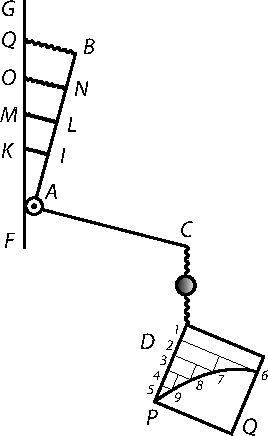
\includegraphics[width=0.34\textwidth]{gesamttex/edit_VIII,3/images/LH_37_03_073-074_d11.pdf}}%\\
%  \vspace*{-2.0em}
%  \centerline{\hspace*{-85mm}\lbrack\textit{Fig.~11}\rbrack}%
%  \label{LH_37_03_074v_d11}%
%  \edtext{}{\lemma{\lbrack\textit{Fig.~11}\rbrack}\killnumber\Cfootnote{**************************}}
%  \vspace*{2.0em}%
%
%
%  \vspace*{-19.0em}
%  \centerline{\hspace*{70mm}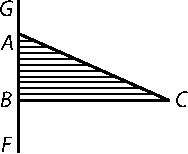
\includegraphics[width=0.23\textwidth]{gesamttex/edit_VIII,3/images/LH_37_03_073-074_d12.pdf}}%\\
%  \vspace*{-0.50em}
%  \centerline{\hspace*{70mm}\lbrack\textit{Fig.~12}\rbrack}%
%  \label{LH_37_03_074v_d12}%
%  \edtext{}{\lemma{\lbrack\textit{Fig.~12}\rbrack}\killnumber\Cfootnote{**************************}}
%  \vspace*{12.5em}%
%
%
% \pstart%
\edtext{Ponamus
\edtext{ergo rectam\protect\index{Sachverzeichnis}{recta rigida} rigidam}{%
\lemma{ergo}\Bfootnote{%
\textit{(1)}~nunc corpus r
\textit{(2)}~rectam rigidam%
~\textit{L}}}
%
\textit{AB} esse applicatam immobili \textit{FG}\protect\index{Sachverzeichnis}{immobile} in \textit{AQ}
annexamque funibus\protect\index{Sachverzeichnis}{funis tensus}
seu chordis,\protect\index{Sachverzeichnis}{chorda tensa}}{%
\lemma{Ponamus \lbrack...\rbrack\ chordis}\Cfootnote{%
Siehe \lbrack\textit{Fig.~11}\rbrack\ auf S.~\pageref{LH_37_03_074v_d11}.??}}
%
quae non sint tensae,
sed in statu suo naturali\protect\index{Sachverzeichnis}{status naturalis}
quando \textit{AB} applicatur ipsi \textit{AQ};
sed quando nisu ponderis \textit{D}\protect\index{Sachverzeichnis}{nisus ponderis}
\edtext{recta}{%
\lemma{recta}\Bfootnote{%
\textit{erg.~L}}}
%
ab \textit{AQ} dimovetur ad situm \textit{AB},
\edtext{tunc}{%
\lemma{tunc}\Bfootnote{%
\textit{erg.~L}}}
%
tendi chordas\protect\index{Sachverzeichnis}{chorda tensa}
ex \textit{Q} in \textit{B}, ex \textit{O} in \textit{N}, ex \textit{M} in \textit{L}, ex \textit{K}
\edtext{in \textit{I}.
Pondus\protect\index{Sachverzeichnis}{pondus tendens} autem \textit{D} dividamus in partes
quae aequivaleant singulae singulis tensionibus,\protect\index{Sachverzeichnis}{tensio chordae}
nempe \textit{126}}{%
\lemma{in}\Bfootnote{%
\hspace{-0,5mm}\textit{I}.
\textit{(1)}~Eritque tensio \textit{QB} ad tensionem \textit{ML} ut \textit{AB} ad \textit{AL}. Jam et si tensiones
\textit{(2)}~Eruntque tensiones \textit{QB}. \textit{ON}. \textit{ML}. \textit{KI} ut rectae
\textit{(3)}~Pondus autem \lbrack...\rbrack\ in partes
\textbar~aequales \textit{gestr.}~%
\textbar\ quae aequivaleant \lbrack...\rbrack\ tensionibus, nempe
\textit{(a)}~\textit{426}
\textit{(b)}~\textit{126}%
~\textit{L}}}
%
ipsi tensioni \textit{QB},
ita ut solum pondus \textit{126}
sustinere possit chordam \textit{QB}\protect\index{Sachverzeichnis}{chorda tensa} in ea tensione,
similiter pondus \textit{237} aequivaleat tensioni
%
\edtext{\textit{ON}, et pondus \textit{348} tensioni \textit{ML},
et pondus\protect\index{Sachverzeichnis}{pondus tendens}
\lbrack\textit{459}\rbrack\
tensioni\protect\index{Sachverzeichnis}{tensio chordae}
\lbrack\textit{KI}\rbrack\
et}{%
\lemma{\textit{ON},}\Bfootnote{%
\textit{(1)}~\textit{348}
\textit{(2)}~et pondus \lbrack...\rbrack\ et pondus % \textit{348} tensioni \textit{ML},
\textbar~\textit{KI} \textit{ändert Hrsg.}~%
\textbar\ tensioni
\textbar~\textit{459} \textit{ändert Hrsg.}~%
\textbar\ et%
~\textit{L}}}
%
ita porro.
Quaeritur\lbrack,\rbrack\
posito \textit{12345} cadere in
\edtext{rectam, et \textit{26. 37. 48. 59}}{%
\lemma{rectam,}\Bfootnote{%
\hspace{-0,5mm}et
\textit{(1)}~pondera particularia
\textit{(2)}~\textbar\ et \textit{streicht Hrsg.}~\textbar\ \textit{26. 37. 48. 59}%
~\textit{L}}}
%
esse parallelas,
\edtext{distantiasque earum \textit{12} et \textit{23} et \textit{34} et \textit{45} esse aequales}{%
\lemma{distantiasque}\Bfootnote{%
\hspace{-0,5mm}earum \lbrack...\rbrack\ esse aequales % \textit{12} et \textit{23} et \textit{34} et \textit{45}
\textit{erg.~L}}}\lbrack,\rbrack\
%
quaenam futura sit curva\protect\index{Sachverzeichnis}{curva}
in quam incident omnia puncta \textit{9876},
seu
\edtext{quae sit ratio\protect\index{Sachverzeichnis}{ratio ponderum} ponderum}{%
\lemma{quae}\Bfootnote{%
\hspace{-0,5mm}sit
\textit{(1)}~ea
\textit{(2)}~ord
\textit{(3)}~pon
\textit{(4)}~ratio ponderum%
~\textit{L}}}
%
tensionibus in hoc situ aequivalentium.\protect\index{Sachverzeichnis}{pondus tendens}
Et quidem Tensio \textit{QB}
\edtext{est}{%
\lemma{est}\Bfootnote{\textit{erg.~L}}}
%
ad tensionem \textit{ON} ut \textit{AB} ad \textit{AN}.
\edtext{Sed etsi tensiones\protect\index{Sachverzeichnis}{tensio chordae}}{%
\lemma{Sed}\Bfootnote{%
\textit{(1)}~licet ten
\textit{(2)}~etsi tensiones%
~\textit{L}}}
%
\textit{QB} et \textit{ON} ponerentur aequales,
tamen quia \textit{ON} centro \textit{A} propior, quam \textit{QB},
eo facilius pondere ex \textit{C} suspenso\protect\index{Sachverzeichnis}{pondus suspensum}
\edtext{vincetur, in ratione propinquitatis ad centrum,}{%
\lemma{vincetur,}\Bfootnote{%
\textit{(1)}~et posito \textit{AC} aequalem esse ipsi \textit{AB}, pondus
\textit{(2)}~id est si ponatur \textit{AC} aequalis ipsi \textit{AB} pondus quod sustinere tensionem
\textit{(3)}~in ratione propinquitatis ad centrum,%
~\textit{L}}}
%
ergo
\edtext{resistentia\protect\index{Sachverzeichnis}{resistentia chordae} chordae \textit{ON}}{%
\lemma{resistentia}\Bfootnote{%
\textit{(1)}~tensionis \textit{ON}
\textit{(2)}~chordae \textit{ON}%
~\textit{L}}}
%
ad resistentiam chordae \textit{QB},\protect\index{Sachverzeichnis}{resistentia chordae}
est in composita
\edtext{ratione\protect\index{Sachverzeichnis}{ratio composita} ex rationibus
tensionum \textit{ON}, et \textit{QB},\protect\index{Sachverzeichnis}{ratio tensionum}}{%
\lemma{ratione}\Bfootnote{%
\hspace{-0,5mm}\textbar~ex rationibus \textit{erg.}~%
\textbar\ tensionum
\textit{(1)}~et \textit{QB}
\textit{(2)}~\textit{ON}, et \textit{QB},%
~\textit{L}}}
%
et rationibus\protect\index{Sachverzeichnis}{ratio distantiarum} distantiarum \textit{AN}, \textit{AB}.
\edtext{Sed tensiones\protect\index{Sachverzeichnis}{tensio chordae}
sunt etiam in ratione}{%
\lemma{Sed}\Bfootnote{%
\textit{(1)}~rationes
\textit{(2)}~tensionem
\textit{(3)}~tensiones sunt etiam in ratione%
~\textit{L}}}
%
distantiarum,\protect\index{Sachverzeichnis}{ratio distantiarum}
ergo resistentia chordae \textit{ON} ad resistentiam chordae \textit{QB}\protect\index{Sachverzeichnis}{resistentia chordae}
erit in duplicata ratione\protect\index{Sachverzeichnis}{ratio duplicata} \textit{AN} ad \textit{AB} seu
\edtext{in ratione quadrati}{%
\lemma{in}\Bfootnote{%
\hspace{-0,5mm}ratione
\textit{(1)}~quadratorum
\textit{(2)}~quadrati%
~\textit{L}}}
%
\textit{AN} ad quadratum
\edtext{\textit{AB}.
%
Ergo et in figura ipsius \textit{D} erunt ordinatae \textit{26}, \textit{37}
inter se ut quadrata abscissarum \textit{P2}, \textit{P3},
adeoque figura\protect\index{Sachverzeichnis}{figura}}{%
\lemma{\textit{AB}.}\Bfootnote{%
\textit{(1)}~Si
\textit{(2)}~Ergo erit et \textit{26} ad \textit{37} in ratione quadratorum abscissae
\textit{(a)}~et
\textit{(b)}~et in figura
\textit{(3)}~Ergo et \lbrack...\rbrack\ adeoque figura% in figura ipsius \textit{D} erunt ordinatae \textit{26}, \textit{37} inter se ut quadrata abscissarum $\textit{P2}, \textit{P3},
~\textit{L}}}
%
ipsius \textit{D} erit trilineum\protect\index{Sachverzeichnis}{trilineum parabolicum} parabolicum concavum,
quod cum sit tertia pars rectanguli circumscripti\protect\index{Sachverzeichnis}{rectangulum circumscriptum}
\textit{1PQ} vim\protect\index{Sachverzeichnis}{vis rumpens}
\edtext{quae directe}{%
\lemma{quae}\Bfootnote{%
\textit{(1)}~totum
\textit{(2)}~directe%
~\textit{L}}}
%
rumperet repraesentantis,
sequitur pondus circulariter rumpens\protect\index{Sachverzeichnis}{pondus circulariter rumpens}
esse tertiam partem ponderis directe rumpentis,\protect\index{Sachverzeichnis}{pondus directe rumpens}
si ex distantia \textit{AC} suspendatur quae sit
\edtext{aequalis longitudini ipsius \textit{AB}.%
\edlabel{LH_37_03_074r-v_EinDrittel_bvxycjw-2}}{%
\lemma{aequalis}\Bfootnote{%
\textit{(1)}~longitudinis
\textit{(2)}~longitudini ipsius
\textit{(a)}~abrumpendi a
\textit{(b)}~abrum
\textit{(c)}~\textit{AB}.%
~\textit{L}}}
%
\pend%
%
\pstart%
Et\edlabel{LH_37_03_074v_TrabsTriangularis_tucbv-1} proinde
cum summae parabolarum quadraticarum\protect\index{Sachverzeichnis}{parabola quadratica} sint ut cubi,
hinc resumendo
\edtext{Calculum\protect\index{Sachverzeichnis}{calculus}}{%
\lemma{Calculum}\Cfootnote{%
Siehe S.~\refpassage{LH_37_03_073v_calculus-1}{LH_37_03_073v_calculus-2}.}}
%
\edtext{figurae 4\protect\index{Sachverzeichnis}{figura}}{\lemma{figurae 4}\Cfootnote{%
\lbrack\textit{Fig.~5}\rbrack\ auf S.~\pageref{LH_37_03_073v_Fig.5}.}}
%
atque huc accommodando,
fiet:
$\displaystyle x\!\!\int\!\!\overline{y\,d\overline{x}}\, - \!\!\int\!\!\overline{yx\,d\overline{x}}$
aequ.\rule[0mm]{0pt}{5,0mm}
$\displaystyle\frac{c}{a}y^3$
et proinde
$\displaystyle \ovalbox{$xy\,d\overline{x}$}+d\overline{x}\!\!\int\!\!\overline{y\,d\overline{x}}-\ovalbox{$xy\,d\overline{x}$}$
aequ.\rule[0mm]{0pt}{5,0mm}
%
\edtext{$\displaystyle\frac{3c}{a}yy\,d\overline{y}$
seu
$\displaystyle\!\!\int\!\!\overline{d\overline{x}\!\!\int\!\!\overline{y\,d\overline{x}}}$
aequ. $y^3.$
Sit \textit{x} aequ. $n\cdot y^h$ et fiet $d\overline{x}$
aequ. $nh\cdot y^{h-1}d\overline{y}$ et $y\,d\overline{x}$
erit $nh\cdot y^hd\overline{y}$}{%
\lemma{$\displaystyle\frac{3c}{a}yy\,d\overline{y}$}\Bfootnote{%
\textit{(1)}~faciamus \textit{y} aequ. $n\cdot x^h$ fiet: \textit{yy} aequ. $nn\cdot x^{2h}$ et $d\overline{y}$ aequ.
\textit{(2)}~seu $\displaystyle\!\!\int\!\!\overline{d\overline{x}\!\!\int\!\!\overline{y\,d\overline{x}}}$
\lbrack...\rbrack\
aequ. $n\cdot y^h$
\textit{(a)}~fiet $d\overline{x}$
\textit{(b)}~et fiet $d\overline{x}$
\lbrack...\rbrack\
erit $nh\cdot y^hd\overline{y}$%
~\textit{L}}}
%
et
$\displaystyle\!\!\int\!\!\overline{y\,d\overline{x}}$
erit\rule[0mm]{0pt}{5,0mm}
$\displaystyle\frac{nh}{h+1}\cdot y^{h+1}$
et
$\displaystyle d\overline{x}\!\!\int\!\!\overline{y\,d\overline{x}}$
erit:% \rule[0mm]{0pt}{6,0mm}
$\displaystyle\frac{nh}{h+1}y^{h+1}\cdot nh\cdot y^{h-1}d\overline{y}.$
Ergo $\displaystyle d\overline{x}\!\!\int\!\!\overline{y\,d\overline{x}}$
erit:\rule[0mm]{0pt}{5,0mm}
$\displaystyle\frac{nnhh}{h+1}y^{2h}d\overline{y}.$
Et
$\displaystyle\!\!\int\!\!\overline{d\overline{x}\!\!\int\!\!\overline{y\,d\overline{x}}}$
erit
% \edtext{}{% überflüssige Variante !!!!
% \lemma{$\displaystyle\frac{nnhh}{h+1}y^{2h}dy.$}\Bfootnote{%
% \textit{(1)}~et $\displaystyle\!\!\int\!\!\overline{d\overline{x}\!\!\int\!\!\overline{y\,d\overline{x}}}$ erit
% \textit{(2)}~et $\displaystyle\!\!\int\!\!\overline{d\overline{x}\!\!\int\!\!\overline{y\,d\overline{x}}}$ erit%
% ~\textit{L}}}
%
% \rule[0mm]{0pt}{5,0mm}%
$\displaystyle\frac{nnhh}{h+1}\!\!\int\!\!\overline{y^{2h}\,d\overline{y}}$
seu % \rule[0mm]{0pt}{6,0mm}
$\displaystyle\frac{nnhh}{\overline{h+1} \cdot \overline{2h+1}}y^{2h+1}$%
\protect\rule[0mm]{0pt}{6mm}aequ.
\edtext{$\displaystyle\frac{c}{a}y^3.$
Quae aequatio debet}{%
\lemma{$\displaystyle\frac{c}{a}y^3.$}\Bfootnote{%
\textit{(1)}~Et fa
\textit{(2)}~Quae aequatio debet%
~\textit{L}}}
%
esse identica,
% \rule[0mm]{0pt}{5,5mm}
itaque 
\pend
\newpage%%%%%künstlicher Seitenumbruch mitten im Absatz KZEITZ
\pstart
\noindent
erit
$2h+1$ aequ. $3,$ seu \textit{h} aequ. $1.$
Porro
$\displaystyle\frac{nnhh}{\overline{h+1} \cdot \overline{2h+1}}$
aequ. % \rule[0mm]{0pt}{5,5mm}
$\displaystyle\frac{c}{a}.$
Ergo fiet \textit{ann} aequ. $6c$
\edtext{et:
\textit{n} aequ. $\displaystyle\sqrt{\protect\vphantom{\protect\mathstrut{\frac{6c}{a}}}}\frac{6c}{a},$
eritque}{%
\lemma{et}\Bfootnote{%
\textit{(1)}~fiet 
\textit{(2)}~: \textit{n} aequ. $\displaystyle\sqrt{\protect\vphantom{\protect\mathstrut{\frac{6c}{a}}}}\frac{6c}{a},$ eritque%
~\textit{L}}}
%
\textit{x} aequ. $\displaystyle\sqrt{\protect\vphantom{\protect\mathstrut{\frac{6c}{a}}}}\frac{6c}{a}.$
Unde patet % \rule[0mm]{0pt}{5,5mm}
lineam quaesitam\protect\index{Sachverzeichnis}{linea quaesita} fore rectam,
seu\rule[0mm]{0pt}{5,0mm}
\edtext{Triangulum rectangulum\protect\index{Sachverzeichnis}{traingulum rectangulum}
\edtext{\textit{BAC}}{%
\lemma{\textit{BAC}}\Bfootnote{ %
\textit{erg.~L}}}
%
muro\protect\index{Sachverzeichnis}{murus}
\edtext{\textit{FG}}{%
\lemma{\textit{FG}}\Bfootnote{%
\textit{erg.~L}}}
%
infixum,}{\lemma{Triangulum \lbrack...\rbrack\ infixum}\Cfootnote{%
Siehe \lbrack\textit{Fig.~12}\rbrack\ auf S.~\pageref{LH_37_03_074v_d12}.??}}
%
atque inde projectum,\rule[0mm]{0pt}{5,0mm}
ubique aequaliter resistere,\protect\index{Sachverzeichnis}{trabs aequiresistens}
nec proinde pondere suo frangi.%
\edlabel{LH_37_03_074v_TrabsTriangularis_tucbv-2}%
\edlabel{LH_37_03_074r_zweiterTeil_lbhuno-2}%
%
\pend
\pstart \vspace{2em} \setline{1}\noindent
\begin{minipage}[t]{0.5\textwidth}
\hspace{10mm}
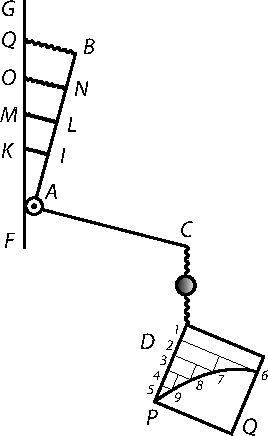
\includegraphics[width=0.64\textwidth]{gesamttex/edit_VIII,3/images/LH_37_03_073-074_d11.pdf}
\end{minipage}
\hspace{23mm}
\begin{minipage}[t]{0.5\textwidth}
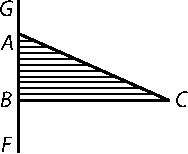
\includegraphics[width=0.47\textwidth]{gesamttex/edit_VIII,3/images/LH_37_03_073-074_d12.pdf}
\end{minipage}
\\
\\
\vspace{1.5em}
\hspace{23mm} [\textit{Fig.~11}] \label{LH_37_03_074v_d11}\hspace{60mm} [\textit{Fig.~12}] \label{LH_37_03_074v_d12}
%\vspace{1em}
\pend

%
%
%
%
%\vspace{1em}
%  \centerline{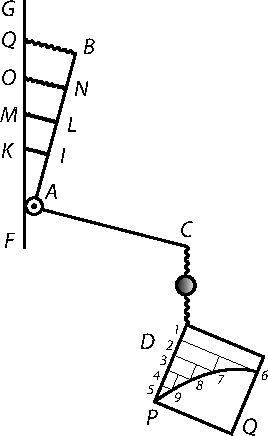
\includegraphics[width=0.32\textwidth]{gesamttex/edit_VIII,3/images/LH_37_03_073-074_d11.pdf}}%\\
%  \vspace{0.5em}
%  \centerline{\lbrack\textit{Fig.~11}\rbrack}%
%  \label{LH_37_03_074v_d11}%
%%  \edtext{}{\lemma{\lbrack\textit{Fig.~11}\rbrack}\killnumber\Cfootnote{**************************}}
%%  \vspace*{2.0em}%
%\pstart
 \count\Bfootins=1200
\count\Afootins=1200
\count\Cfootins=1200
%\vspace{1em}
%\pend
%  \centerline{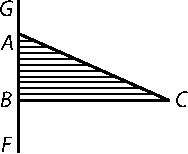
\includegraphics[width=0.22\textwidth]{gesamttex/edit_VIII,3/images/LH_37_03_073-074_d12.pdf}}%\\
%  \vspace{0.50em}
%  \centerline{\lbrack\textit{Fig.~12}\rbrack}%
%  \label{LH_37_03_074v_d12}
% %
%%  \edtext{}{\lemma{\lbrack\textit{Fig.~12}\rbrack}\killnumber\Cfootnote{**************************}}
%  \vspace*{0.0em}%
%
%
%
% ENDE DES STÜCKS AUF BLATT 74v
%
%
% \newpage%
%
%